\documentclass[12pt,a4 paper] {report}
\renewcommand{\familydefault}{\sfdefault}
\usepackage[english]{babel}
\usepackage{microtype}
\usepackage{graphicx}
\usepackage{index}
\usepackage{enumitem}
\usepackage{fixltx2e}
\usepackage{geometry}
\geometry{a4paper , tmargin=3cm , bmargin=2cm , lmargin=2cm , rmargin=2cm}

\title{
	\textbf{S4\_VHDL Specifications} \\
	\begin{figure}[h]
		\centering
		
\includegraphics[scale=0.4]{../png/rwu.png}
	\end{figure}
	Circuit Design (WS2020/21) \\
	Prof. Dr. -Ing Andreas Siggelkow \\
}
\author{Nils Schlegel, 32067 \& Tara Jaishi, 32289}
\date{17.01.2021}


\begin{document}
\maketitle

\newpage

\begin{center}
	\begin{tabular}{llr}
		\multicolumn{3}{l}{\textbf{History - Change Log}} \\
		\hline
		Target Spec. & \multicolumn{2}{l}{Current version: 1.0, 2021-01-17} \\
		& \multicolumn{2}{l}{Previous version: 0.1, 2020-11-9} \\
		\hline
		&	17.01.2021 & FiniteStateMachines added \\
		&	17.01.2021 & Block diagrams created and updated \\
		&	17.01.2021 & Block descriptions added \\
		&	06.11.2020 & General description added \\
		&	06.11.2020 & Block diagram added \\
		&	06.11.2020 & Functional description added \\
		&	06.11.2020 & Document created
	\end{tabular}
\end{center}

\newpage

\tableofcontents

\newpage

\chapter{General discription}
IC4 is a single chip based application containing processing capabilities to detect and keep track of the amount of people in one room. It is part of a system solution to fullfill the covid-19-restrictions and regulate the amount of people in an area. This solution is only meant for a chamber with only one doorway available to enter or to exit.\newline
The IC4 is designed on a FPGA prototype-board Max1000 with 10M16SAU169C8G device on board.
\newpage	
\section{Block diagram}
\begin{figure}[h]
	\centering	
	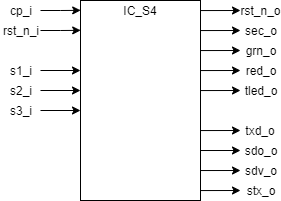
\includegraphics[scale=0.6]{../png/top.png}
\end{figure}

\newpage

\chapter{Requirements}
\begin{center}
	\begin{tabular}{|p{1.5cm}|p{3.5cm}|p{2cm}|p{2cm}|p{6cm}|}
		\hline
		\textbf{ID} & \textbf{Requirement} & \textbf{Priority} & \textbf{Verifiable} & \textbf{Description}\\
		\hline
		\multicolumn{5}{|l|}{\textbf{General}} \\
		\hline
		G01 & Gen.: \#persons &  High &  Testbench & The number of persons in a room must be known. \\
		\hline
		G02 & Gen.: max & High &  Testbench & The number of persons in a room must not exceed a given limit. \\
		\hline
		G03 & Gen.: only one pers. & High & ? & Only one person can either enter or leave the room at a time. \\
		\hline
		G04 & Gen.: three light sensors & Medium & Testbench & Along the doorway, there are three light-curtains to allow directiontracking of possible visitors. \\
		\hline
		G05 & Gen.: only one door & High & ? & Only one door exists. \\
		\hline
		\multicolumn{5}{|l|}{\textbf{Sound}} \\
		\hline
		S01 & Sound: entered & High & Testbench & A person entered the room, play a unique sound. \\
		\hline
		S02 & Sound: left & High & Testbench & A person left the room, play a unique sound. \\
		\hline
		S03 & Sound: stop & High & Testbench & The room is full, play a unique sound. \\
		\hline
		\multicolumn{5}{|l|}{\textbf{LED}} \\
		\hline
		LED01 & LED: red &  High & Testbench & The maximal number of persons reached. \\
		\hline
		LED02 & LED: green & High & Testbench & The maximal number of persons not reached. \\
		\hline
	\end{tabular}
\end{center}
\begin{center}
	\begin{tabular}{|p{1.5cm}|p{3.5cm}|p{2cm}|p{2cm}|p{6cm}|}
		\hline
		\textbf{ID} & \textbf{Requirement} & \textbf{Priority} & \textbf{Verifiable} & \textbf{Description}\\
		\hline
		\multicolumn{5}{|l|}{\textbf{UART}} \\
		\hline
		UART01 & UART: 9600 baud & High &  Testbench & The speed of the serial transmission should be set to 9600 baud. \\
		\hline
		UART02 & UART: 8 bit & High & Testbench & The data width of the serial transmission should be set to 8 bit. \\
		\hline
		UART03 & UART: no parity & High & Testbench & The serial transmission should not be checked with a parity bit. \\
		\hline
		UART04 & UART: one stop bit & High  & Testbench & The serial transmission should have only one stop bit. \\
		\hline
		UART05 & UART: time & High & Testbench  & The time stamp of an event should be delivered to a PC. \\
		\hline
		UART06 & UART: \#persons & High &  Testbench &  The \#persons should be transmitted to a PC. \\
		\hline
		\multicolumn{5}{|l|}{\textbf{PC}} \\
		\hline	
		PC01 & PC: language & Medium & C++-program &  The information should be displayed on a PC, the language is C++. \\
		\hline
		\multicolumn{5}{|l|}{\textbf{IC\_S3}} \\
		\hline
		IC01 & IC\_S3: interface & Low & Testbench & Use a three wire IF. \\
		\hline
		IC02 & IC\_S3: events & Low & Testbench & All events should be transmitted via the three wire IF. \\
		\hline
		IC03 & IC\_S3: \#persons & Low  & Testbench & The \#persons should be transmitted via the three wire IF. \\
		\hline
	\end{tabular}
\end{center}

\newpage

\chapter{Top Level View}
\begin{flushleft}
	rb\_i \hspace{1cm} reset \hfill reset, active low
\end{flushleft} 
cp\_i \hspace{1cm} system clock \hfill e.g. 10MHz \\
s1\_i \hspace{1cm} light\_curtain s1 \hfill log1: something passes \\
s2\_i \hspace{1cm} light\_curtain s2 \hfill log1: something passes \\
s3\_i \hspace{1cm} light\_curtain s3 \hfill log1: something passes \\
grn\_o\hspace{0.9cm}LED, access garanted \hfill Green LED, go ahead \\
red\_o\hspace{0.9cm}LED, stop, no entry \hfill Red LED, stop, access denied \\
sdo\_o\hspace{0.9cm}serial data out \hfill drives S3 or MC\\
sdv\_o\hspace{0.9cm}serial data valid \hfill drives S3 or MC\\
stx\_o\hspace{1cm}serial transfer active \hfill drives S3 or MC\\
txd\_o\hspace{1cm}serial out \hfill to RS-232-driver, 9k6,8N2,ASCII,to PC\\
snd\_o\hspace{0.9cm}sound signal \hfill acoustic signal, to loudspeaker\\
\\
inc\_s \hspace{0.9cm} increment \hfill increments head count when triggered\\
dec\_s \hspace{0.8cm} decrement \hfill decrements head count when triggered\\
num\_s \hspace{0.6cm} number \hfill contains the head count number\\
evh\_s \hspace{0.8cm} event \hfill contains the current event\\

\chapter{Functional description}
\section*{HeadCount}
Stores the current number of people in the room. It increments or decrements the number if needed.
\section*{EventHandler}
It recieves the signals from the light curtains and dectects with event is triggered. Depending on the event it will play a sound, turn on a LED and create an output signal.
\section*{UniqueTime}
This element is only counting the clock-cycles, to generate a unique timestamp. \newpage
\section*{UART}
The connection to RS232 is done by the UART. It takes the unique timestamp from the UART as well as the head count from the HeadCount and event type from the EventHandler, when a signal from the EventHandler is recieved.
\section*{3WireInterface}
The IC\_3 can be connected by using the 3WireInterface. When it recieves a signal from the EventHandler it should pass the head count and event type to the IC\_3.


The ASIC must:\\
• identify, if a person enters or leaves the room\\
• activate or deactivate a "STOP- " or a "GO-LED"\\
• track and count the number of people presently in the room. Events and head-counts are transferred to IC S3 using a three-wire-Interface and via a UART to a PC. \\
• The transmission to the PC is 9600 baud, 8 bit, no parity, 1 stop bit. \\
On the PC side, get the information and display it. The programming language is
C++.\\

\begin{figure}[h]
	\centering	
	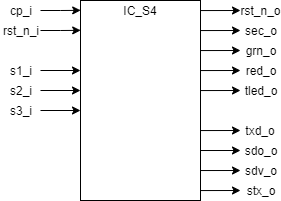
\includegraphics[scale=0.3]{../png/top.png}
	fig: Top level diagram\\
\end{figure}

\newpage

 Table: Top level I/O \\
\begin{center}
	\begin{tabular}{ | p{2cm} | c | c | p{5cm} |}
		\hline
		\textbf{Pin} & \textbf{Direction} & \textbf{Width} & \textbf{Description} \\
		\hline
		rst\_n\_i & IN & 1 & Reset, active low \\
		\hline
		clk\_i & IN & 1 & Syscp, @ 12MHz \\
		\hline
		s1\_i & IN & 3 & Sensor 1 \\
		\hline
		s2\_i & IN & 1 & Sensor 2 \\
		\hline
		s3\_i & IN & 1 & Sensor 3 \\
		\hline
		rst\_n\_o & OUT & 1 & Reset state LED \\
		\hline
		sec\_o & OUT & 1 & Pulse LED \\
		\hline
		grn\_o & OUT & 1 & Green LED \\
		\hline
		red\_o & OUT & 1 & Red LED\\
		\hline
		tled\_o & OUT & 1 & Transmission LED \\
		\hline
		txd\_o & OUT & 1 & Transmission \\
		\hline
		sdi\_o & OUT & 1 & S3 data value \\
		\hline
		sdv\_o & OUT & 1 & S3 data valid \\
		\hline
		stx\_o & OUT & 1 & S3 transmission active \\
		\hline
	\end{tabular}
\end{center}

\newpage

Blocks of Top Level diagram and its Pin and Sifnal are described below. 

\section{Debouncing all Signals}	
\begin{figure}[h]
	\centering	
	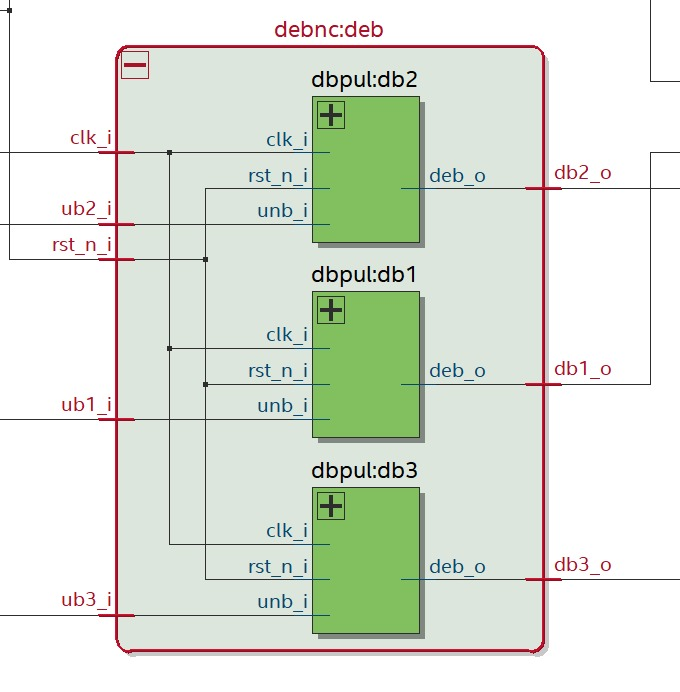
\includegraphics[scale=0.3]{../png/debnc_deb.png}
	\newline
	fig: debnc\_deb \\
\end{figure}

\begin{center}
	\begin{tabular}{ | p{2cm} | c | c | p{5cm} |}
		\hline
		\textbf{Pin} & \textbf{Direction} & \textbf{Width} & \textbf{Description} \\
		\hline
	  rst\_n\_i & IN & 1 & Reset, active low\\
	  \hline
		clk\_i & IN & 1 & Syscp, @ 12MHz \\
		\hline
		ub1\_i & IN & 1 & Unbounced Input 1 \\
		\hline
		ub2\_i & IN & 1 & Unbounced Input 2 \\
		\hline
		ub3\_i & IN & 1 & Unbounced Input 3 \\
		\hline
		db1\_o & OUT & 1 & Debounced Output 1 \\
		\hline
		db2\_o & OUT & 1 & Debounced Output 2 \\
		\hline
		db3\_o & OUT & 1 & Debounced Output 3 \\
		\hline
	\end{tabular}
\end{center}

\newpage

\subsection{Signal Toggle}
\begin{figure}[h]
	\centering	
	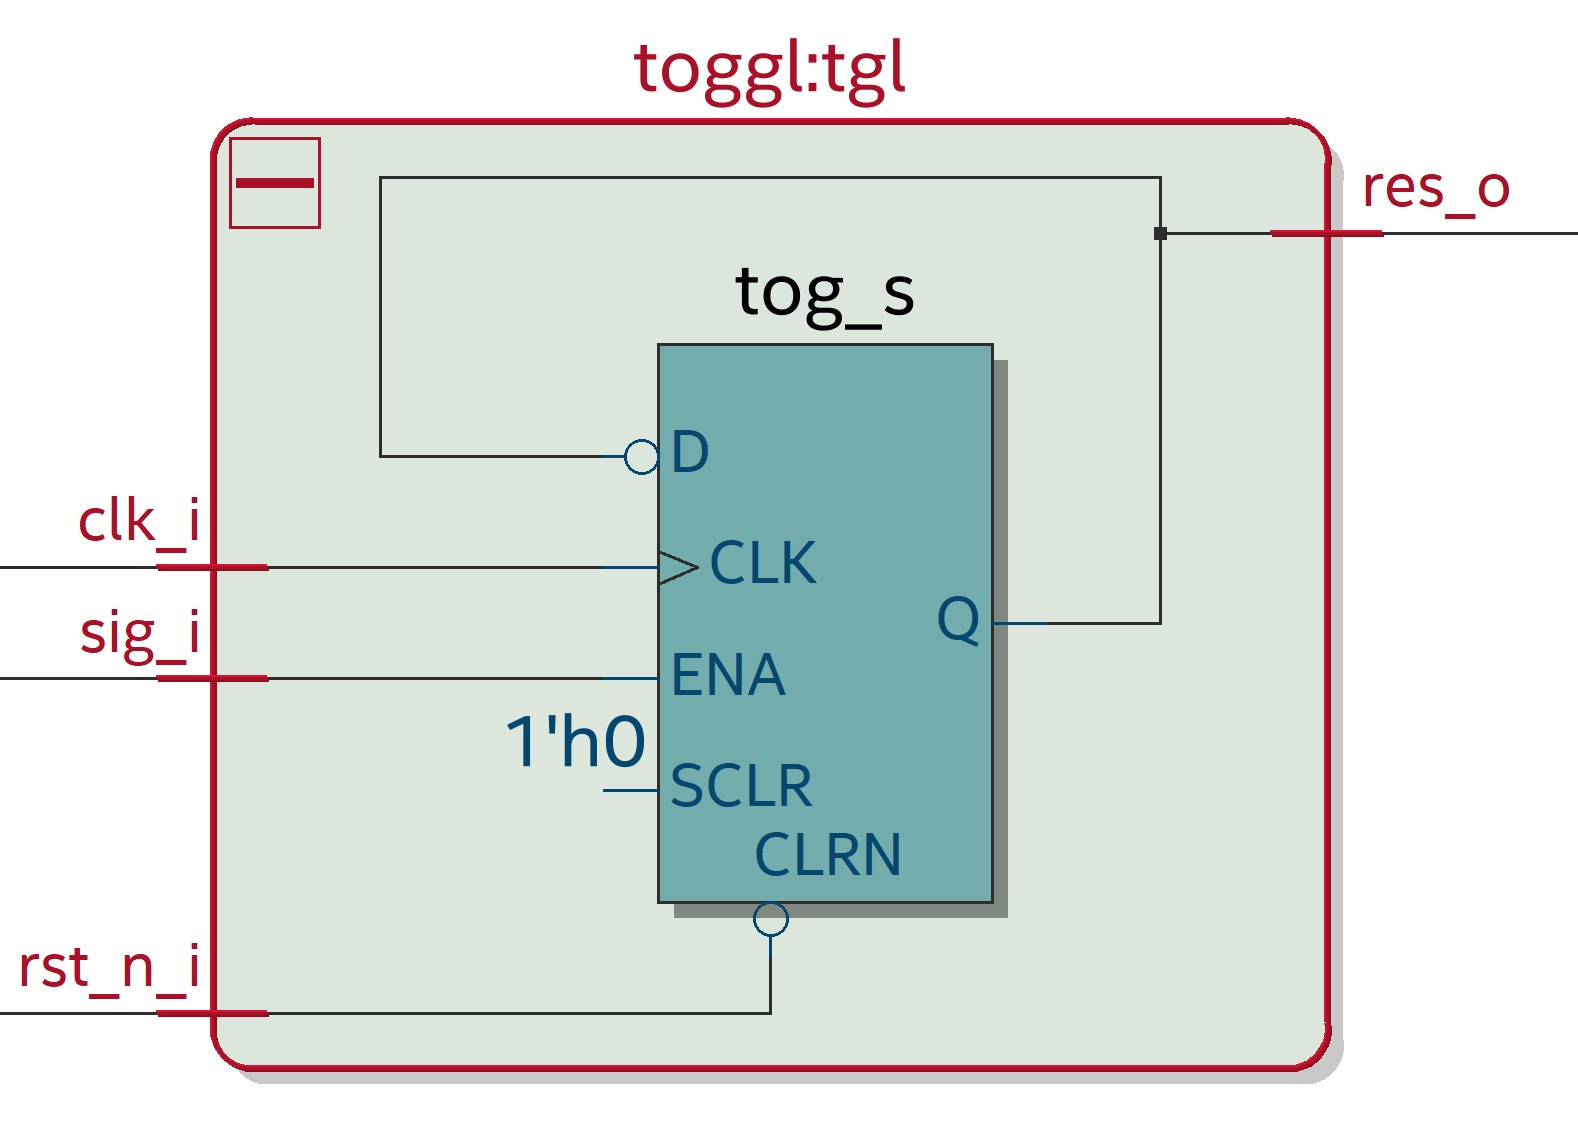
\includegraphics[scale=0.2]{../png/toggl_tgl.png}
	\newline
	fig: toggle\_tgl \\
\end{figure}
\begin{center}
	\begin{tabular}{ | p{2cm} | c | c | p{5cm} |}
		\hline
		\textbf{Pin} & \textbf{Direction} & \textbf{Width} & \textbf{Description} \\
		\hline	
	  rst\_n\_i & IN & 1 & Reset, active low \\
	  \hline
		clk\_i & IN & 1 & Syscp, @ 12MHz \\
		\hline
		sig\_i & IN & 1 & Pulseing signal \\
		\hline
		res\_o & OUT & 1 & Toggeled output \\
		\hline
	\end{tabular}
\end{center}
\newpage
\subsection{Generates Clock Rates}
\begin{figure}[h]
	\centering
	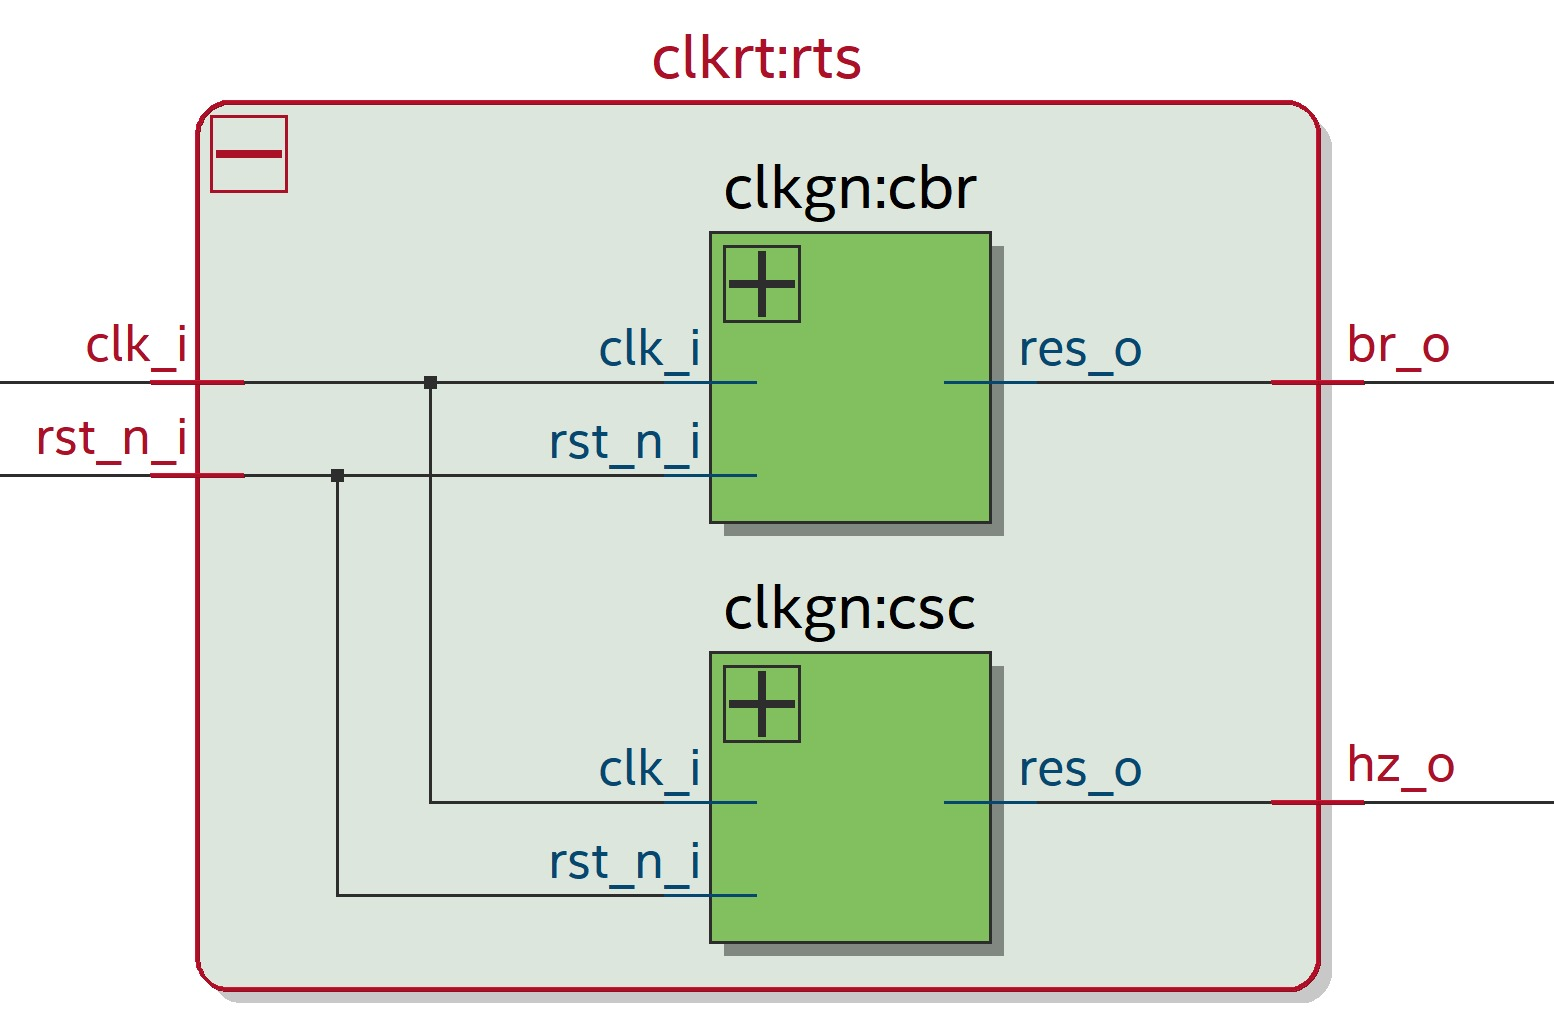
\includegraphics[scale=0.3]{../png/clkrt_rts.png}
	\newline
	fig : clkrt\_rts \\
\end{figure}

\begin{center}
	\begin{tabular}{ | p{2cm} | c | c | p{5cm} |}
		\hline
		\textbf{Pin} & \textbf{Direction} & \textbf{Width} & \textbf{Description} \\
		\hline	
		rst\_n\_i & IN & 1 & Reset, active low \\
		\hline
		clk\_i & IN & 1 & Syscp, @ 12MHz \\
		\hline
		br\_o & OUT & 1 & Baud Rate @9600Hz \\
		\hline
		hz\_o & OUT & 1 & Alive Pulse @1Hz \\
		\hline
	\end{tabular}
\end{center}

\newpage

\subsection{Sensor Handling}
\begin{figure}[h]
	\centering	
	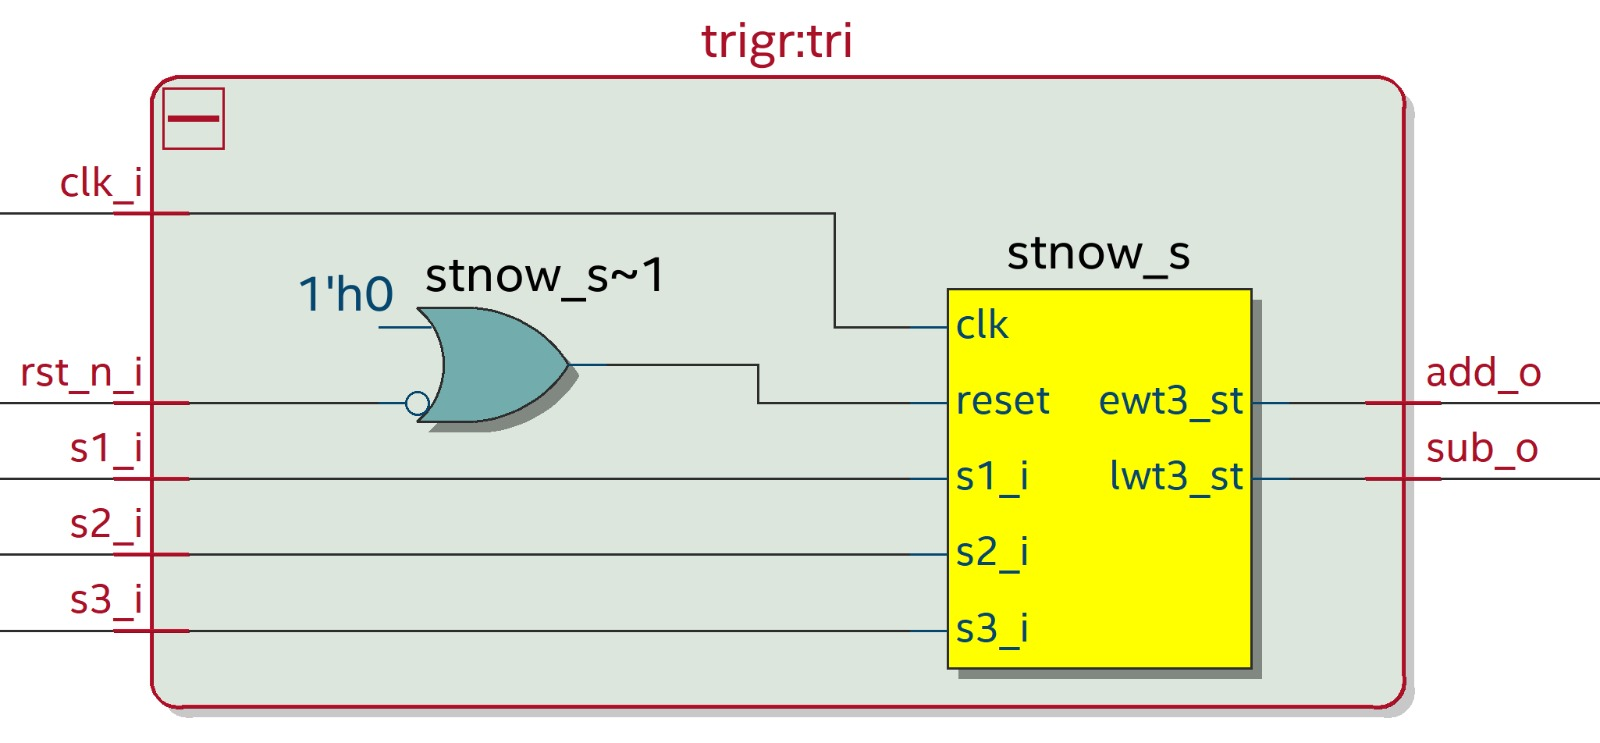
\includegraphics[scale=0.2]{../png/trigr_tri.png}
	\newline
	fig: trigr\_tri \\
\end{figure}
\begin{center}
	\begin{tabular}{ | p{2cm} | c | c | p{5cm} |}
		\hline
		\textbf{Pin} & \textbf{Direction} & \textbf{Width} & \textbf{Description} \\
		\hline	
		rst\_n\_i & IN & 1 & Reset, active low \\
		\hline
		clk\_i & IN & 1 & Syscp, @ 12MHz \\
		\hline
		s1\_i & IN & 1 & Sensor 1 \\
		\hline
		s2\_i & IN & 1 & Sensor 2 \\
		\hline
		s3\_i & IN & 1 & Sensor 3 \\
		\hline
		add\_o & OUT & 1 & Person entered \\
		\hline
		sub\_o & OUT & 1 & Person left \\
		\hline
	\end{tabular}
\end{center}
\newpage

\subsection{HeadCounter}
\begin{figure}[h]
	\centering	
	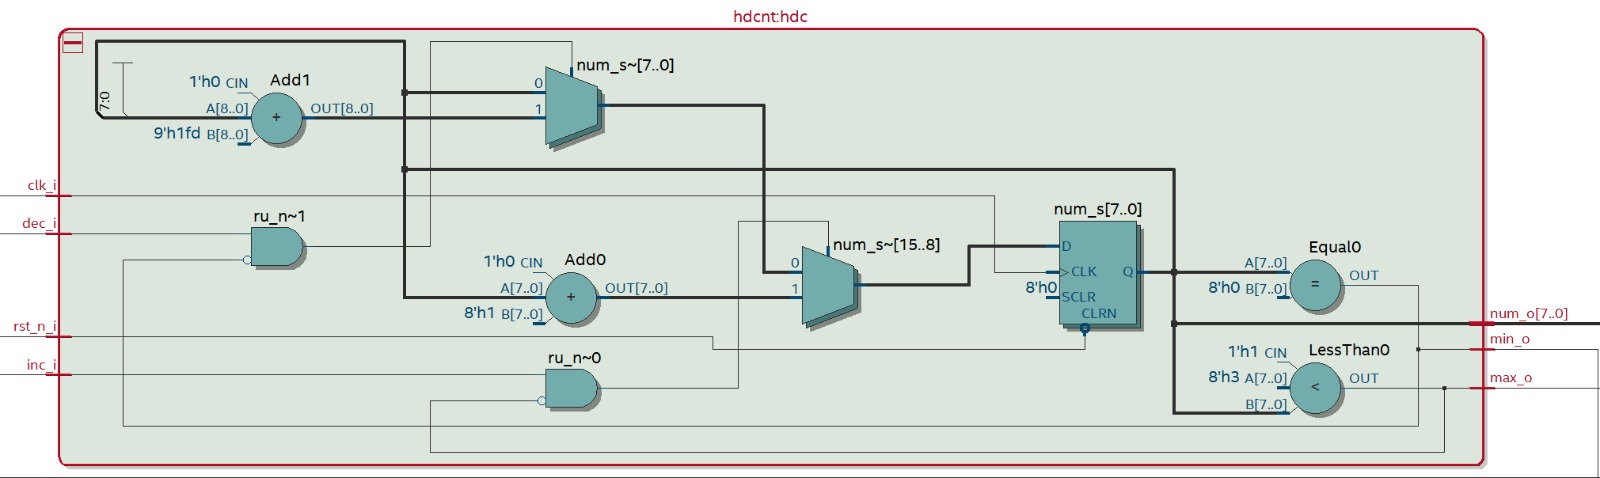
\includegraphics[scale=0.3]{../png/hdcnt_hdc.png}
	\newline
	fig: hdcnt\_hdc \\
\end{figure}
\begin{center}
	\begin{tabular}{ | p{2cm} | c | c | p{5cm} |}
		\hline
		\textbf{Pin} & \textbf{Direction} & \textbf{Width} & \textbf{Description} \\
		\hline	
		rst\_n\_i & IN & 1 & Reset, active low \\
		\hline
		clk\_i & IN & 1 & Syscp, @ 12MHz \\
		\hline
		inc\_i & IN & 1 & Increment Counter Signal \\
		\hline
		dec\_i & IN & 1 & Decrement Counter Signal \\
		\hline
		min\_o & OUT & 1 & Min persons in room \\
		\hline
		max\_o & OUT & 1 & Max persons in room \\
		\hline
		num\_o & OUT &  & \\
		\hline
	\end{tabular}
\end{center}
\begin{center}
	\begin{tabular}{| p{2cm} | p{2cm} | p{4cm} |}
		\hline
		\textbf{Generic} & \textbf{Type} & \textbf{Description} \\
		\hline
		cnt\_width & integer & \\
		\hline
		max\_cnt & integer & \\
		\hline
	\end{tabular}	
\end{center}


\newpage
\subsection{ControllFSM}
\begin{figure}[h]
	\centering	
	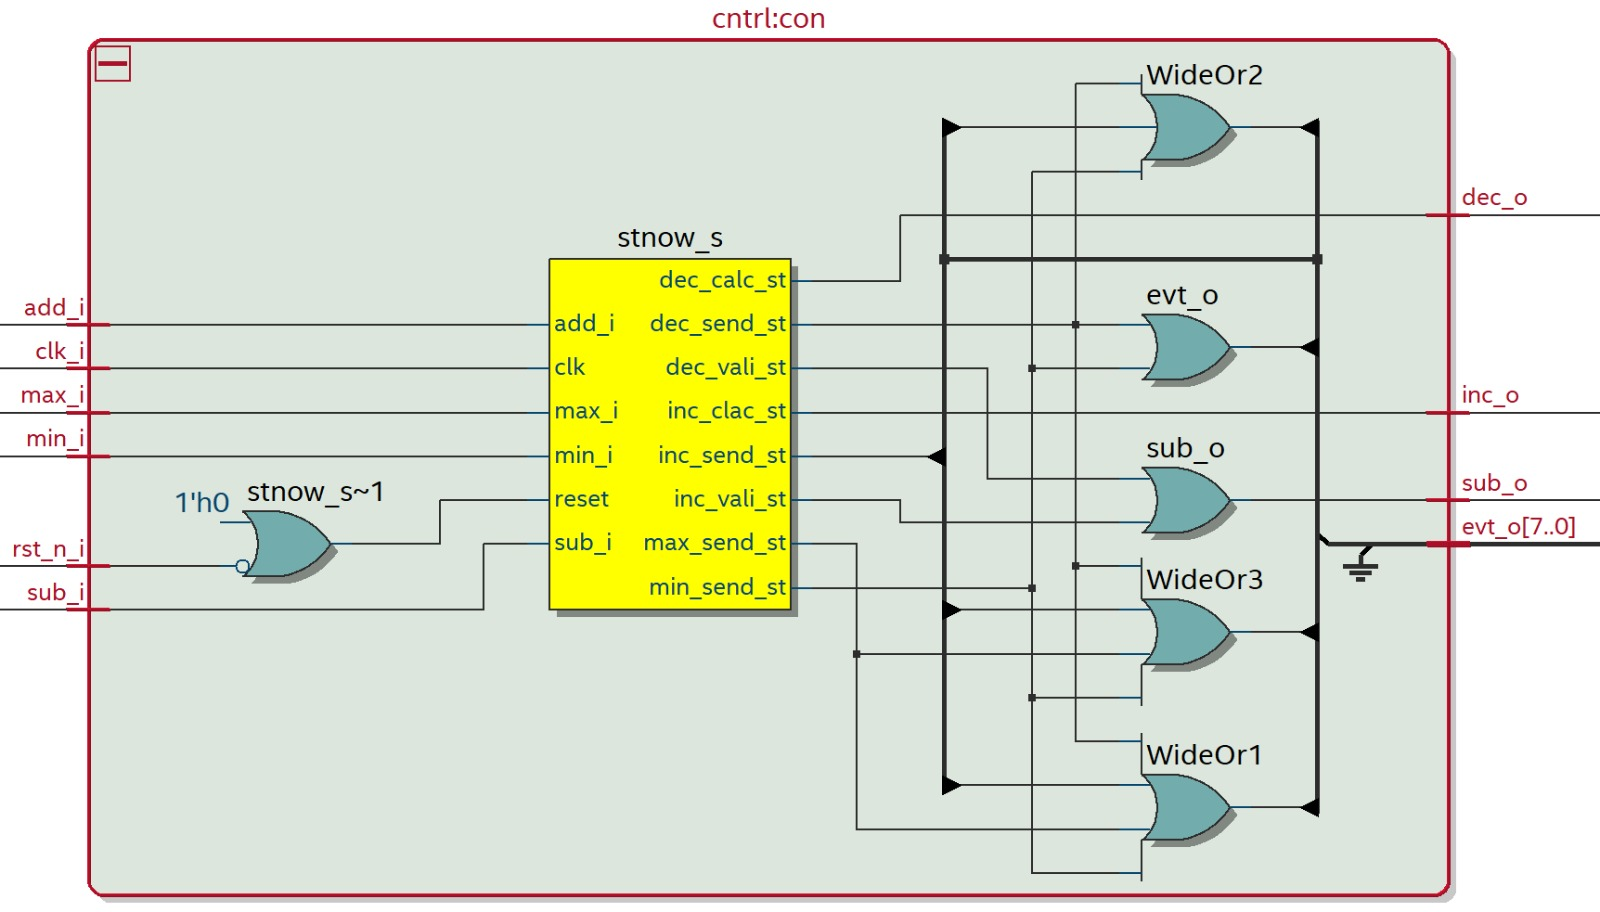
\includegraphics[scale=0.3]{../png/cntrl_con.png}
	\newline
	fig: cntrl\_con \\
\end{figure}
\begin{center}
	\begin{tabular}{ | p{2cm} | c | c | p{5cm} |}
		\hline
		\textbf{Pin} & \textbf{Direction} & \textbf{Width} & \textbf{Description} \\
		\hline	
		rst\_n\_i & IN & 1 & Reset, active low \\
		\hline
		clk\_i & IN & 1 & Syscp, @ 12MHz \\
		\hline
		add\_i & IN & 1 & Person entered \\
		\hline
		sub\_i & IN & 1 & Person left \\
		\hline
		min\_i & IN & 1 & Min persons in room \\
		\hline
		max\_i & IN & 1 & Max persons in room \\
		\hline
		inc\_o & OUT & 1 & Increment Counter Signal \\
		\hline
		dec\_o & OUT & 1 & Decrement Counter Signal \\
		\hline
		evt\_o & OUT &  & Happened event char \\
		\hline
		sub\_o & OUT & 1 & Submitt/Send Data \\
		\hline
	\end{tabular}
\end{center}

\newpage

\subsection{UART to PC}
\begin{figure}[h]
	\centering	
	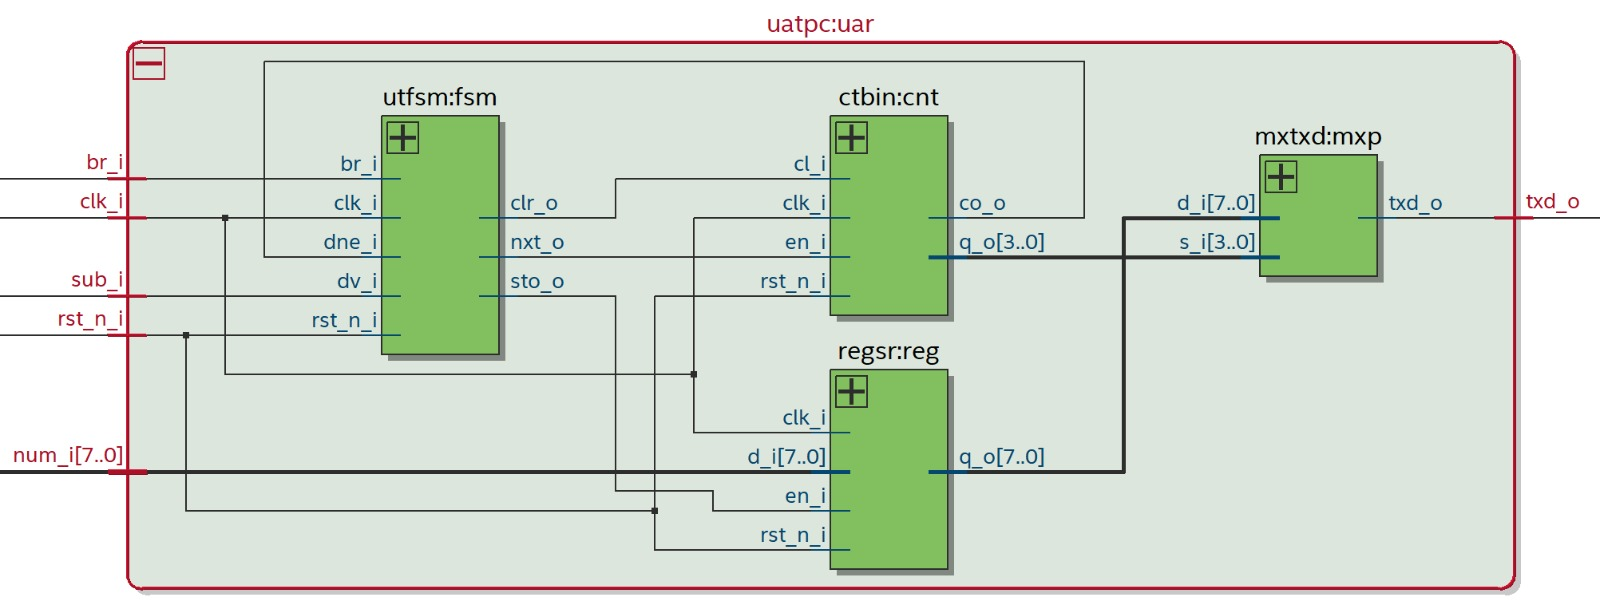
\includegraphics[scale=0.3]{../png/uatpc_uar.png}
	\newline
	fig: uatpc\_uar\\
\end{figure}
\begin{center}
	\begin{tabular}{ | p{2cm} | c | c | p{5cm} |}
		\hline
		\textbf{Pin} & \textbf{Direction} & \textbf{Width} & \textbf{Description} \\
		\hline	
  	rst\_n\_i & IN & 1 & Reset, active low\\
  	\hline
		clk\_i & IN & 1 & Syscp, @ 12MHz \\
		\hline
		br\_i & IN & 1 & Baud rate \\
		\hline
		sub\_i & IN & 1 & Submitt/Send Data \\
		\hline
		num\_i & IN &  & Head count number \\
		\hline
		txd\_o & OUT & 1 & Serial output \\
		\hline
	\end{tabular}
\end{center}

\newpage

\subsection{Interface to S3}
\begin{figure}[h]
	\centering	
	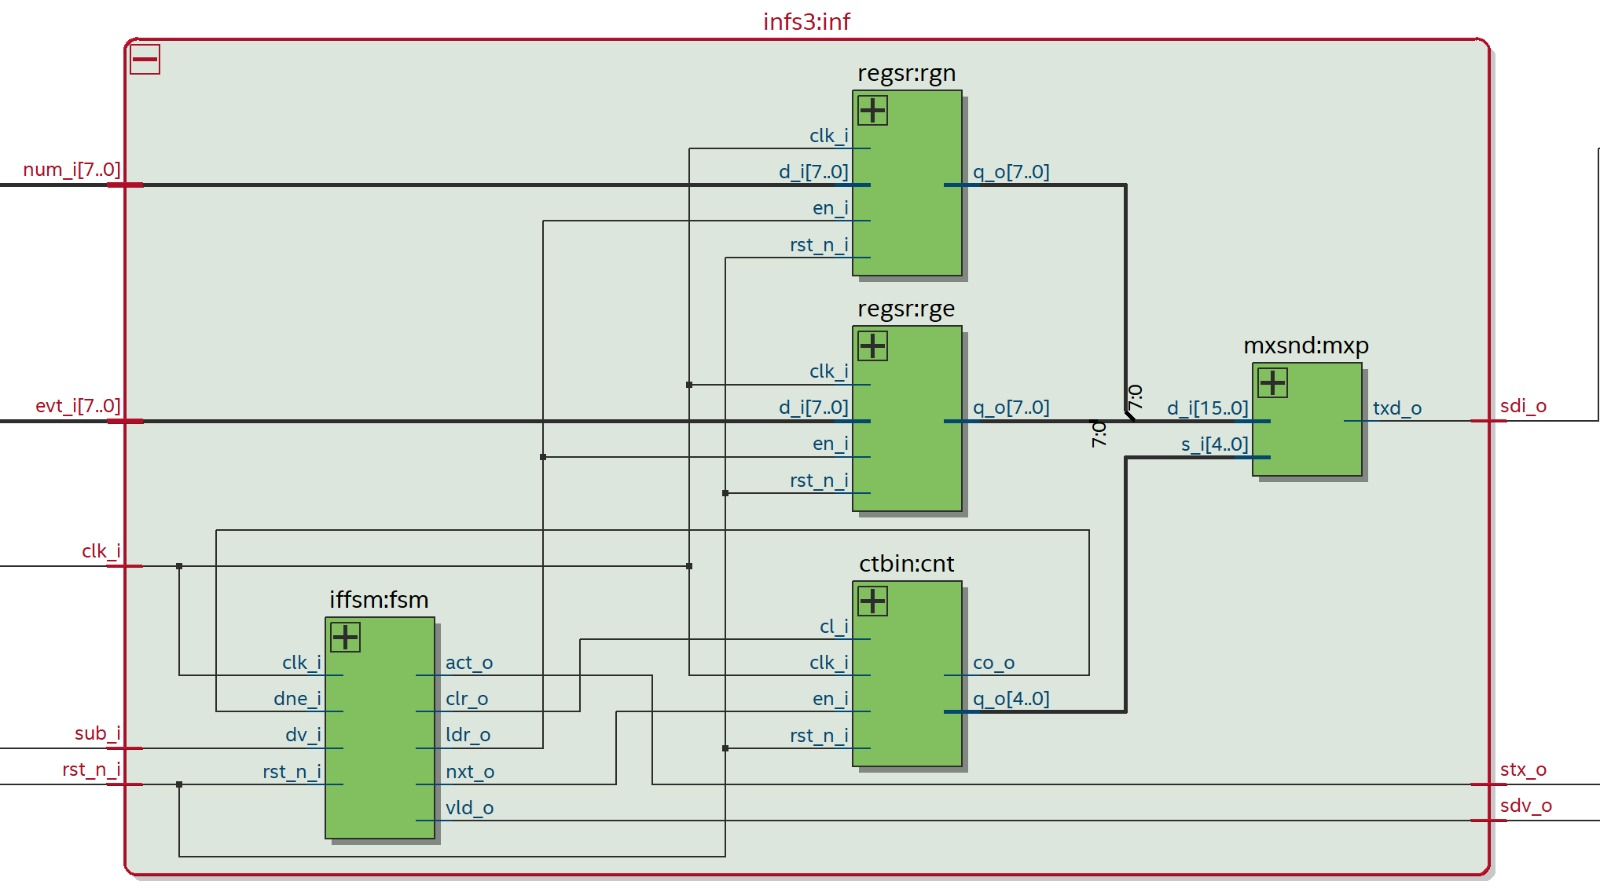
\includegraphics[scale=0.3]{../png/infs3_inf.png}
	\newline
	fig: infs3\_inf\\
\end{figure}
\begin{center}
	\begin{tabular}{ | p{2cm} | c | c | p{5cm} |}
		\hline
		\textbf{Pin} & \textbf{Direction} & \textbf{Width} & \textbf{Description} \\
		\hline	
  	rst\_n\_i & IN & 1 & Reset, active low \\
  	\hline
		clk\_i & IN & 1 & Syscp, @ 12MHz \\
		\hline
		sub\_i & IN & 1 & Submitt/Send Data \\
		\hline
		evt\_i & IN & 1 &  Occured event char \\
		\hline
		num\_i & IN & 1 & Head count number \\
		\hline
		sdi\_o & OUT & 1 & S3 data value \\
		\hline
		sdv\_o & OUT & 1 & S3 data valid \\
		\hline
		stx\_o & OUT & 1 & S3 transmission active\\
		\hline
	\end{tabular}
\end{center}

\newpage

Lower Level Modules are described below.\\
\subsection{Debounc Input resulting in Pulse}
\begin{figure}[h]
	\centering	
	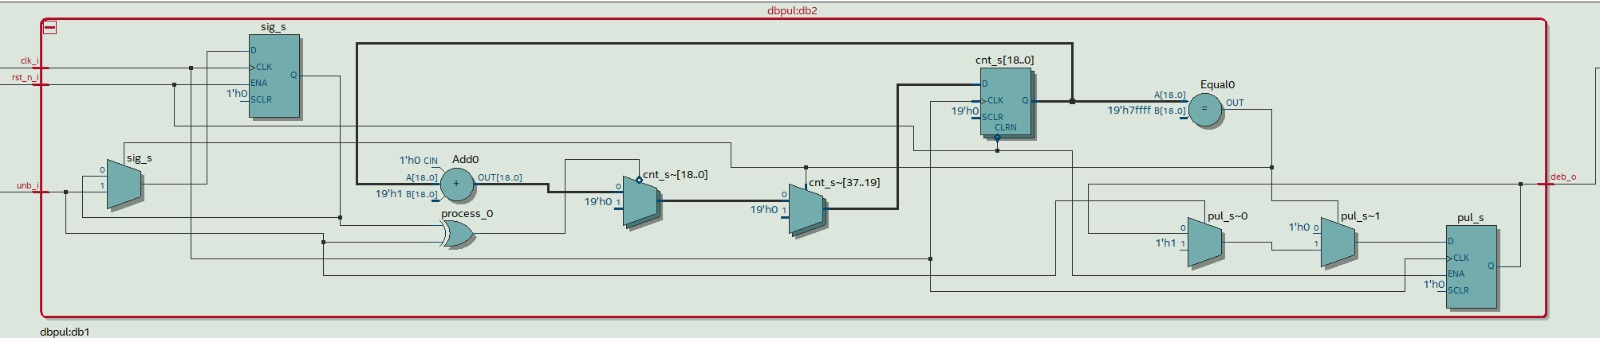
\includegraphics[scale=0.3]{../png/dbpul_db2.png}
	\newline
	fig: dbpul\_db2\\
\end{figure}
\begin{center}
	\begin{tabular}{ | p{2cm} | c | c | p{5cm} |}
		\hline
		\textbf{Pin} & \textbf{Direction} & \textbf{Width} & \textbf{Description} \\
		\hline	
  	rst\_n\_i & IN & 1 &  Reset, active low \\
  	\hline
		clk\_i & IN & 1 & Syscp, @ 12MHz \\
		\hline
		unb\_i & IN & 1 & Unbounced Input \\
		\hline
		deb\_o & OUT & 1 & Debounced Output \\
		\hline
	\end{tabular}
\end{center}
\newpage
\subsection{Clock Generator}
\begin{figure}[h]
	\centering	
	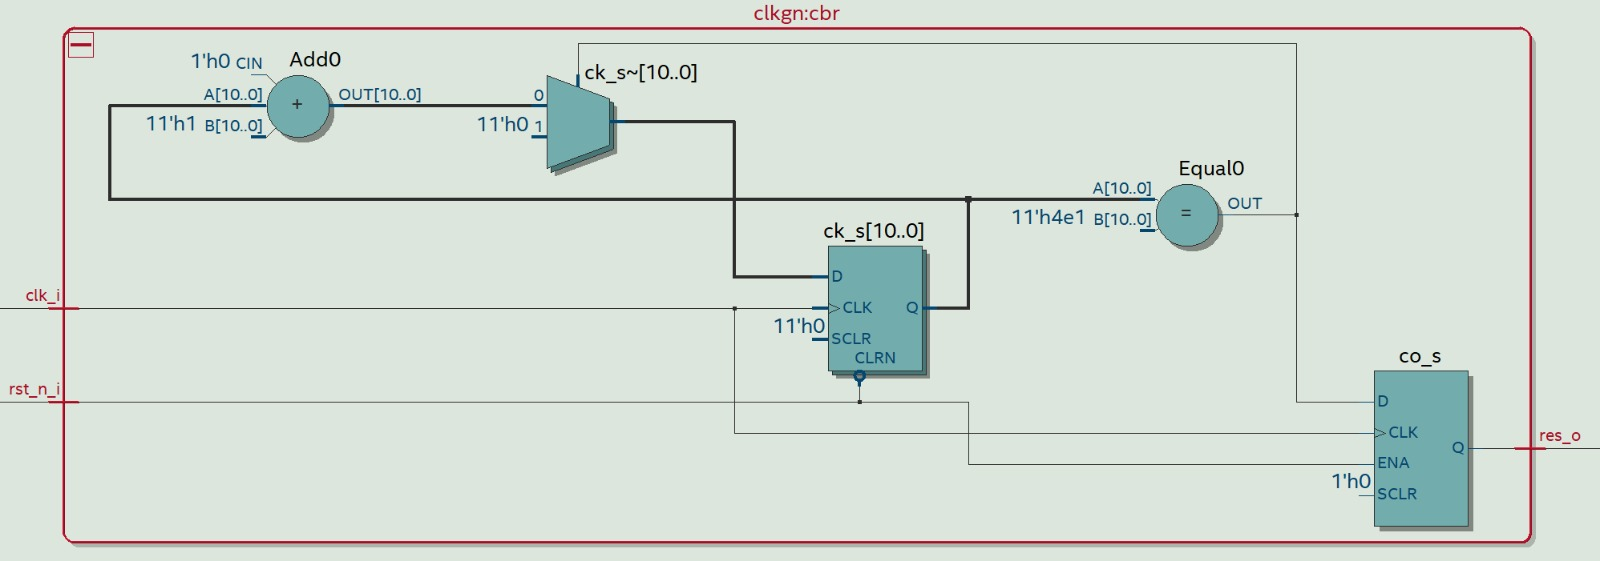
\includegraphics[scale=0.2]{../png/clkgn_cbr.png}
	\newline
	fig: clkgn\_cbr\\
\end{figure}
\begin{figure}[h]
	\centering	
	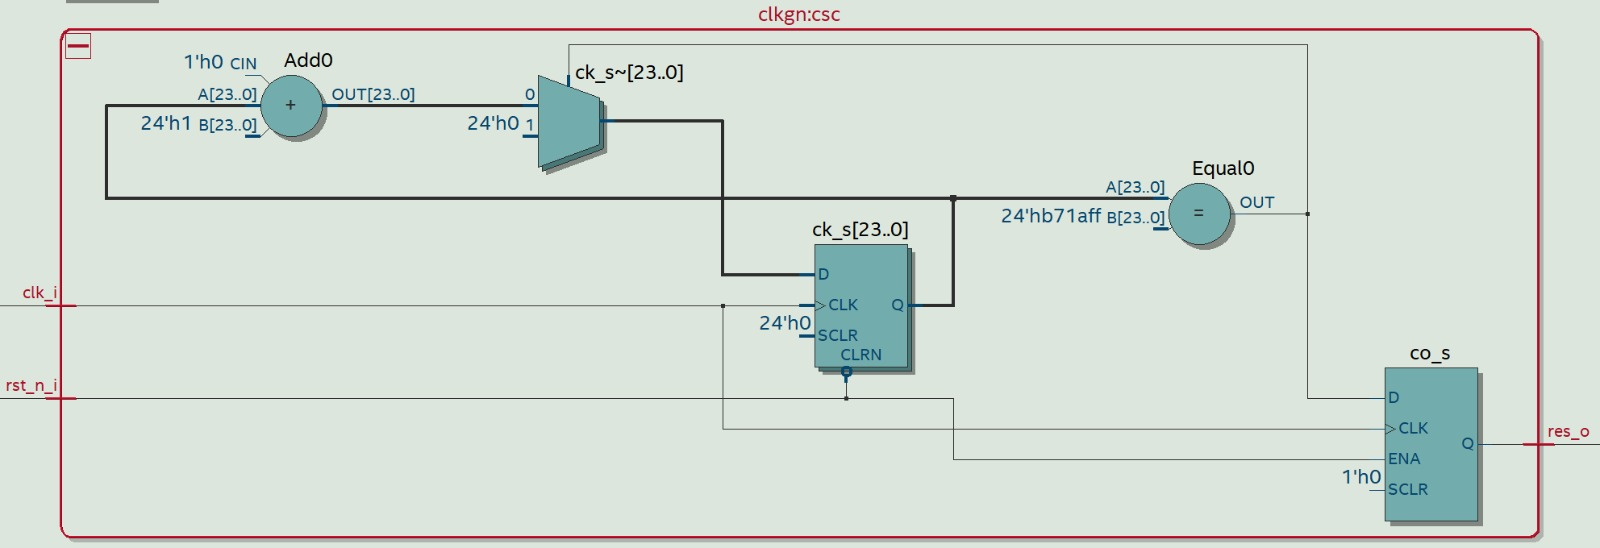
\includegraphics[scale=0.2]{../png/clkgn_csc.png}
	\newline
	fig: clkgn\_csc\\
\end{figure}
\begin{center}
	\begin{tabular}{ | p{2cm} | c | c | p{5cm} |}
		\hline
		\textbf{Pin} & \textbf{Direction} & \textbf{Width} & \textbf{Description} \\
		\hline	
  	rst\_n\_i & IN & 1 & Reset, active low \\
  	\hline
		clk\_i & IN & 1 & Syscp, @ 12MHz \\
		\hline
		res\_o & OUT & 1 & Resulting Ticks \\
		\hline
		
	\end{tabular}
\end{center}
\begin{center}
	\begin{tabular}{| p{2cm} | p{2cm} | p{4cm} |}
	\hline
	\textbf{Generic} & \textbf{Type} & \textbf{Description} \\
	\hline
	cnt\_width & integer & \\
	\hline
	div\_cnt & integer & \\	
	\hline
	\end{tabular}	
\end{center}


\newpage

\subsection{Finite State Machine for UART}
\begin{figure}[h]
	\centering	
	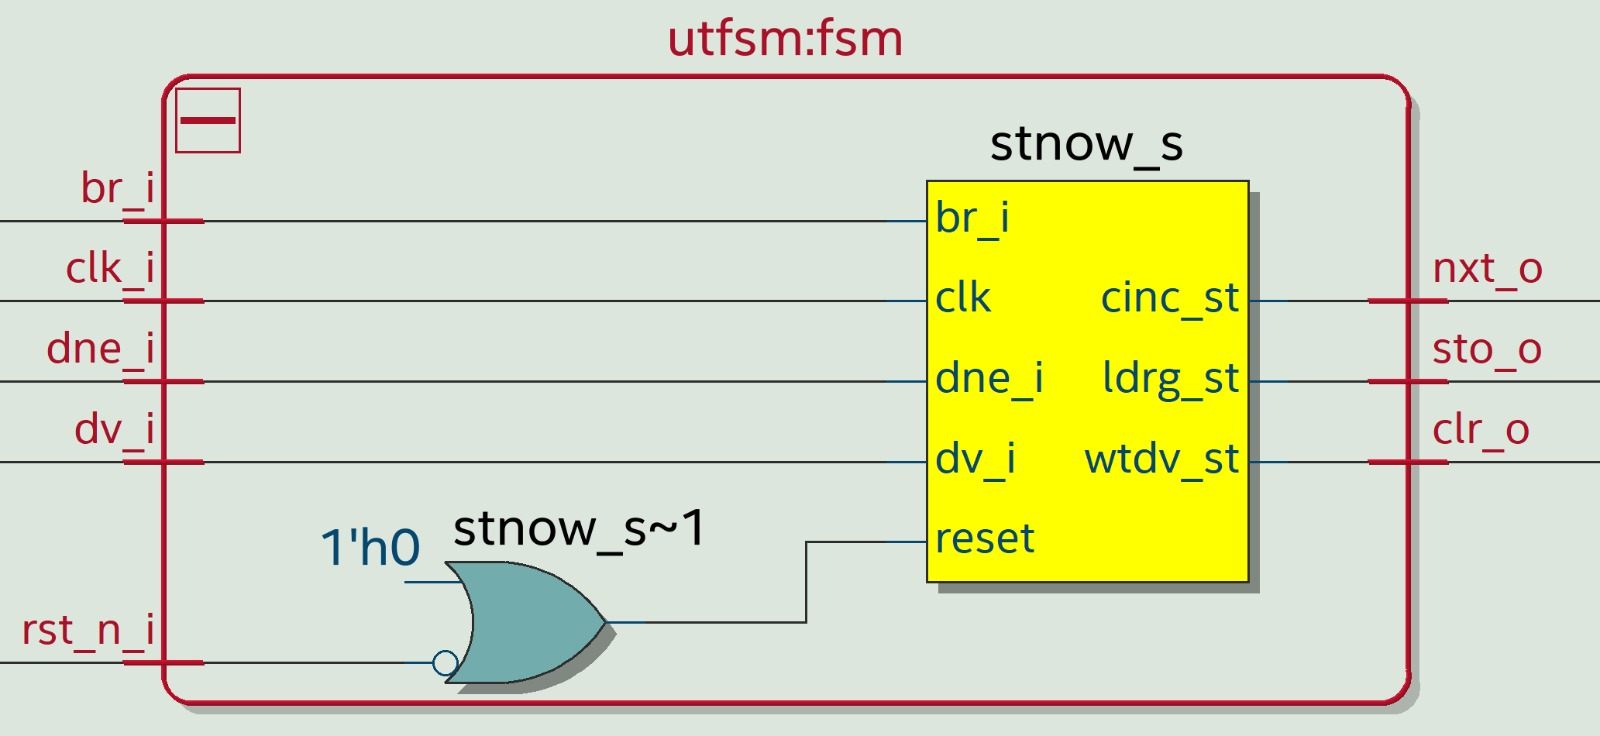
\includegraphics[scale=0.2]{../png/utfsm_fsm.png}
	\newline
	fig: utfsm\_fsm\\
\end{figure}

\begin{center}
	\begin{tabular}{ | p{2cm} | c | c | p{5cm} |}
		\hline
		\textbf{Pin} & \textbf{Direction} & \textbf{Width} & \textbf{Description} \\
		\hline	
		rst\_n\_i & IN & 1 & Reset, active low \\
		\hline
		clk\_i & IN & 1 & Syscp, @ 12MHz \\
		\hline
		dv\_i  & IN & 1 & Have new RTC or GPS-Data \\
		\hline
		br\_i  & IN & 1 & Baud-Rate to ena Counter \\
		\hline
		dne\_i & IN & 1 & Last Bit transmitted \\
		\hline
		sto\_o & OUT & 1 & enable register load \\
		\hline
		clr\_o & OUT & 1 & clear Bit-Counters \\
		\hline
		nxt\_o & OUT & 1 & next Bit, inc count \\
		\hline
		
	\end{tabular}
\end{center}

\newpage

\subsection{Register to store bits}
\begin{figure}[h]
	\centering	
	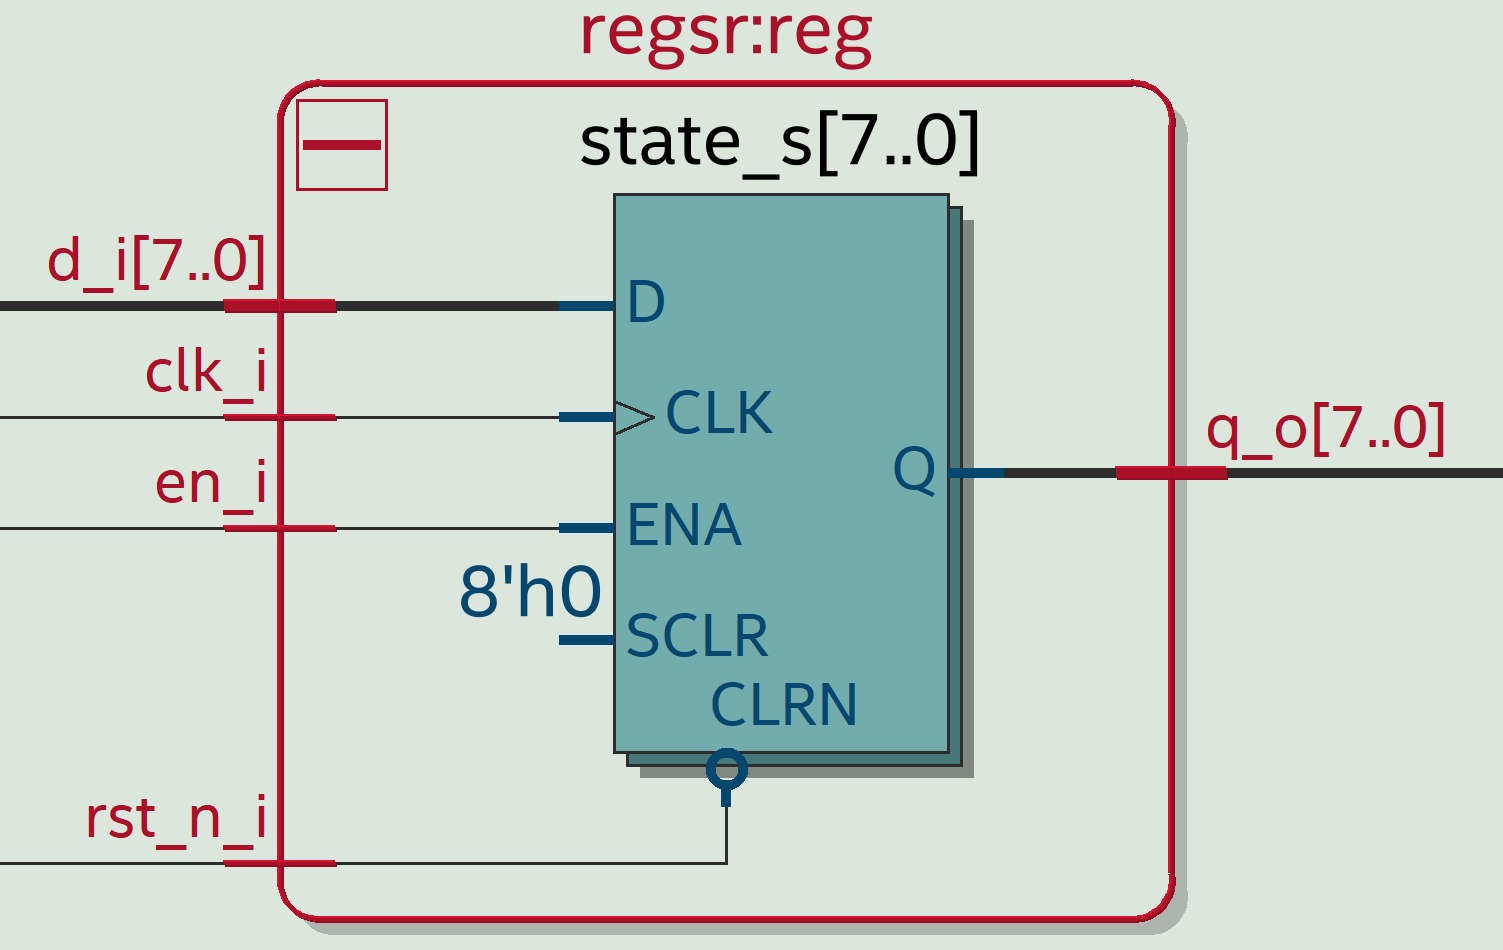
\includegraphics[scale=0.1]{../png/regsr_reg.png}
	\newline
	fig: regsr\_reg\\
\end{figure}
\begin{figure}[h]
	\centering	
	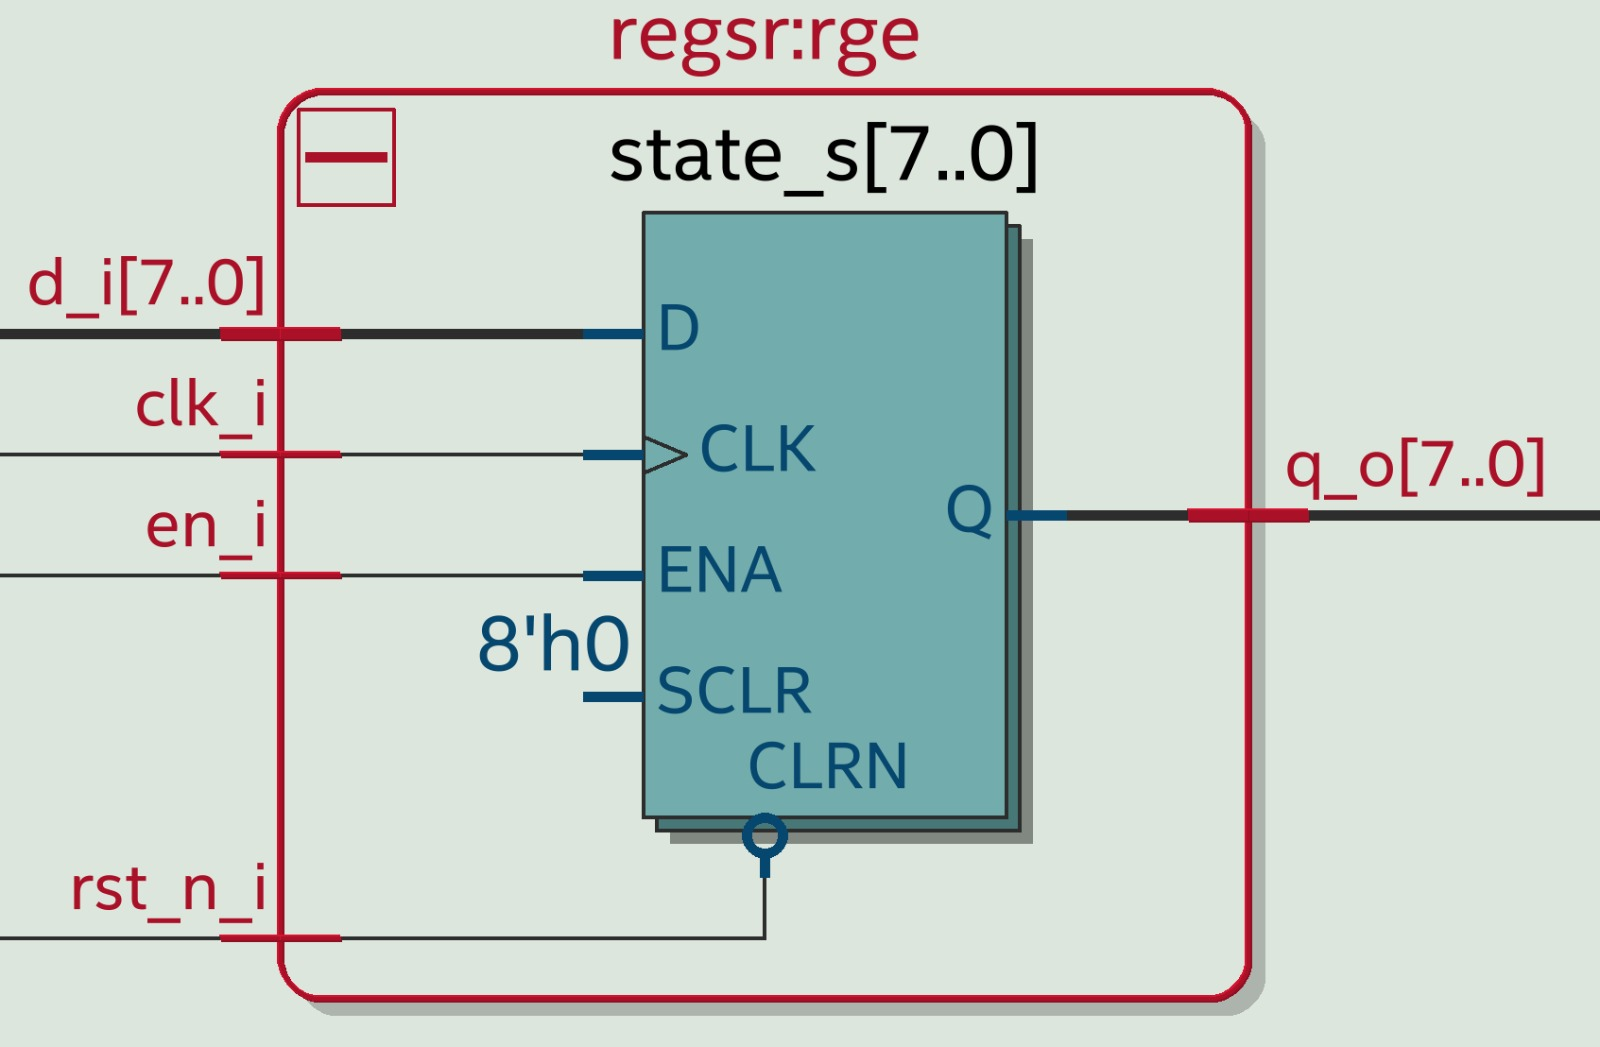
\includegraphics[scale=0.1]{../png/regsr_rge.png}
	\newline
	fig: regsr\_rge\\
\end{figure}
\newpage
\begin{figure}[h]
	\centering	
	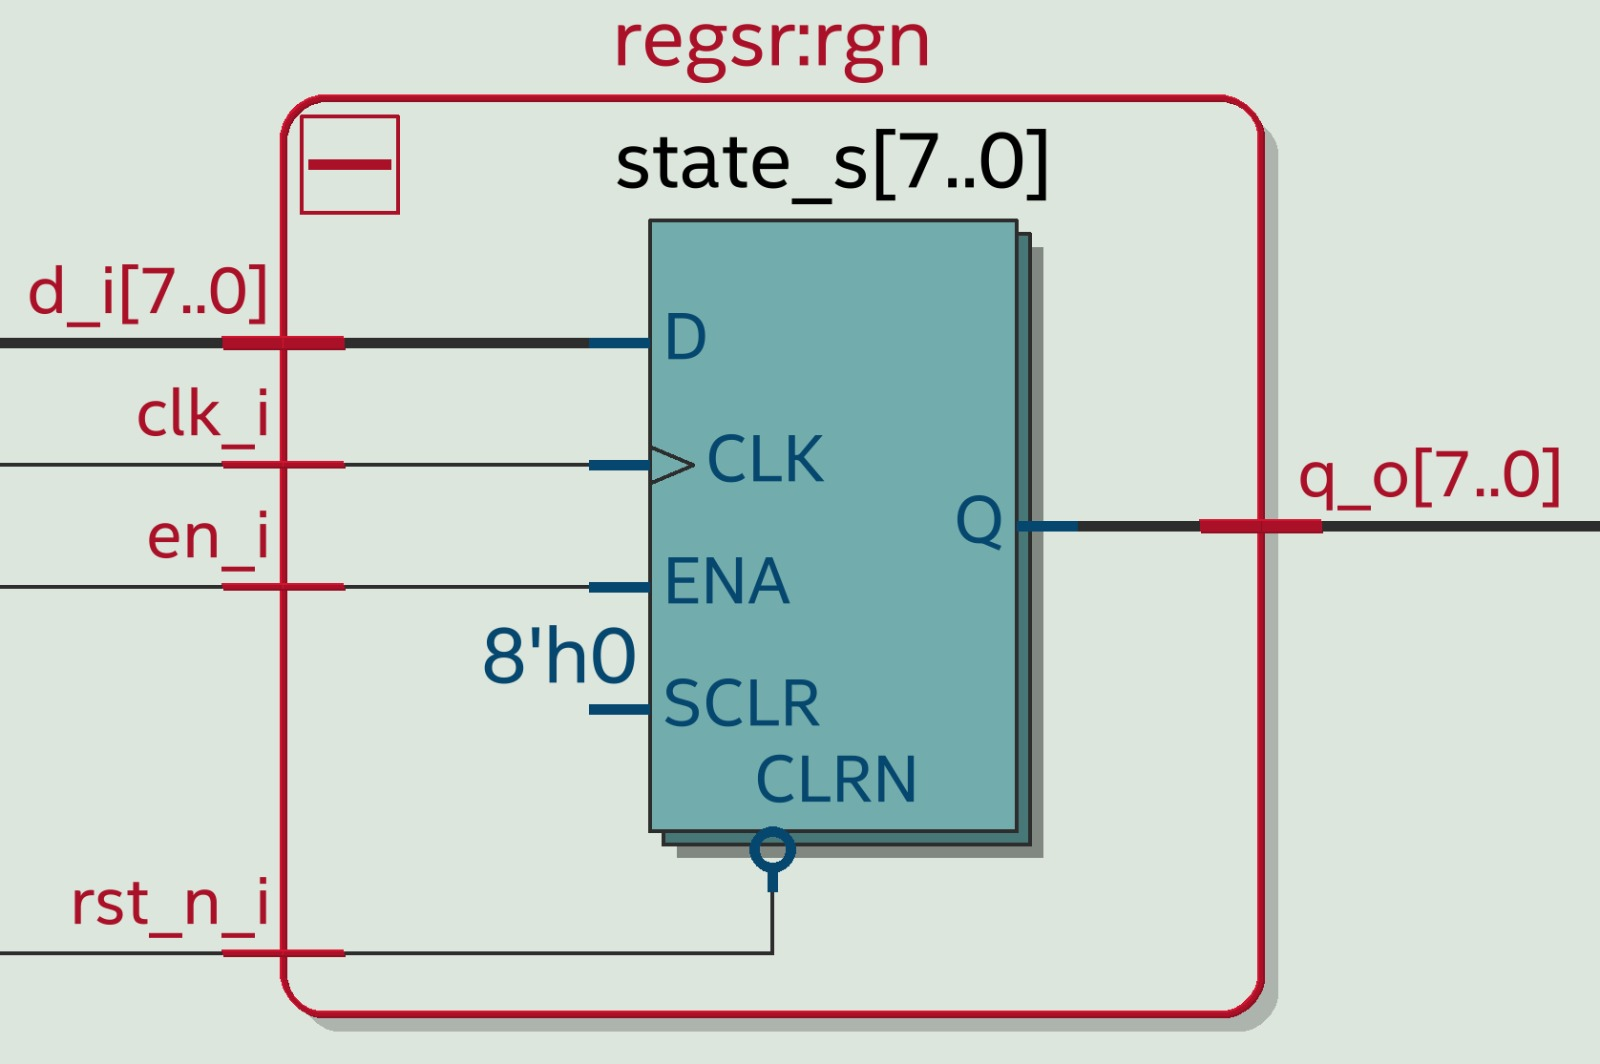
\includegraphics[scale=0.2]{../png/regsr_rgn.png}
	\newline
	fig: regsr\_rgn\\
\end{figure}
dta\_width : integer\\
\begin{center}
	\begin{tabular}{ | p{2cm} | c | c | p{5cm} |}
		\hline
		\textbf{Pin} & \textbf{Direction} & \textbf{Width} & \textbf{Description} \\
		\hline	
 		rst\_n\_i & IN & 1 & Reset, active low \\
 		\hline
		clk\_i & IN & 1 & Syscp, @ 12MHz \\
		\hline
		en\_i & IN & 1 & Store Data \\
		\hline
		d\_i & IN & 1 & Input Data \\
		\hline
		q\_o & OUT & 1 & Stored Data \\
		\hline
		
	\end{tabular}
\end{center}



\newpage
\subsection{Binary Counter}
\begin{figure}[h]
	\centering	
	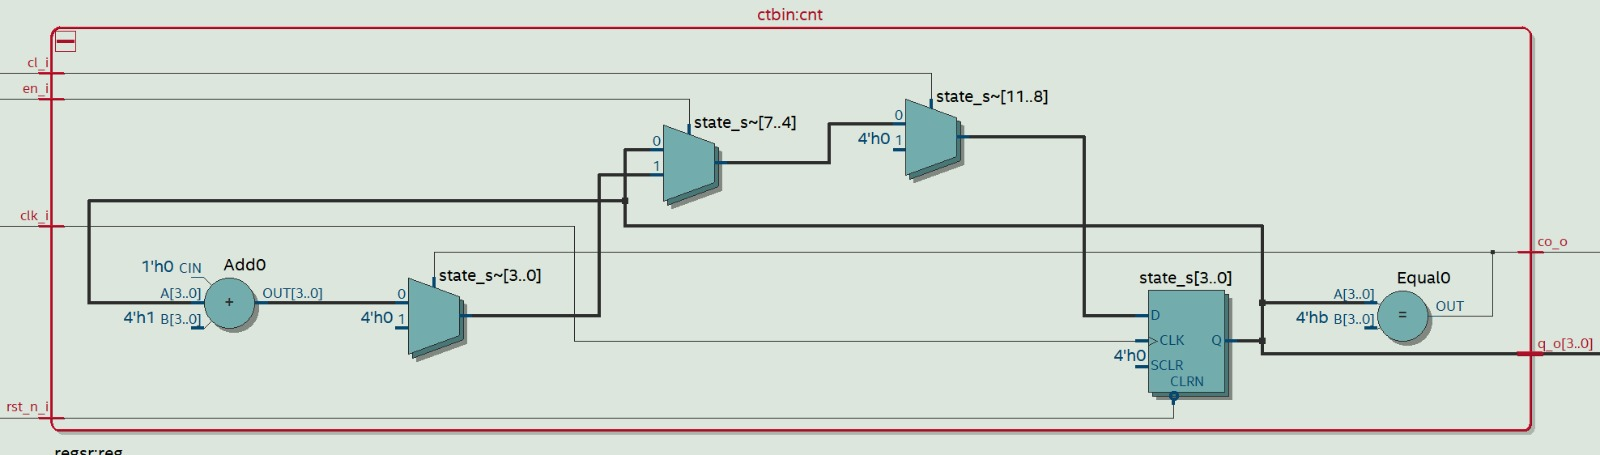
\includegraphics[scale=0.2]{../png/ctbin_cnt.png}
	\newline
	fig:ctbin\_cnt\\
\end{figure}
\begin{center}
	\begin{tabular}{| p{2cm} | p{2cm} | p{4cm} |}
		\hline
		\textbf{Generic} & \textbf{Type} & \textbf{Description} \\
		\hline
 		cnt\_width & integer & \\
		\hline
		cnt\_max & integer & \\
		\hline
	\end{tabular}	
\end{center}

\begin{center}
	\begin{tabular}{ | p{2cm} | c | c | p{5cm} |}
		\hline
		\textbf{Pin} & \textbf{Direction} & \textbf{Width} & \textbf{Description} \\
		\hline	
 		 rst\_n\_i & IN & 1 & Reset, active low \\
 		 \hline
		clk\_i & IN & 1 & Syscp, @ 12MHz \\
		\hline
		en\_i & IN & 1 & Enable Count \\
		\hline
		cl\_i & IN & 1 & Clear Counter \\
		\hline
		co\_o & OUT & 1 & Carry Out \\
		\hline
		q\_o & OUT & 1 & Counter Value \\
		\hline
		
	\end{tabular}
\end{center}
\newpage

\subsection{Multiplexer for TXD}
\begin{figure}[h]
	\centering	
	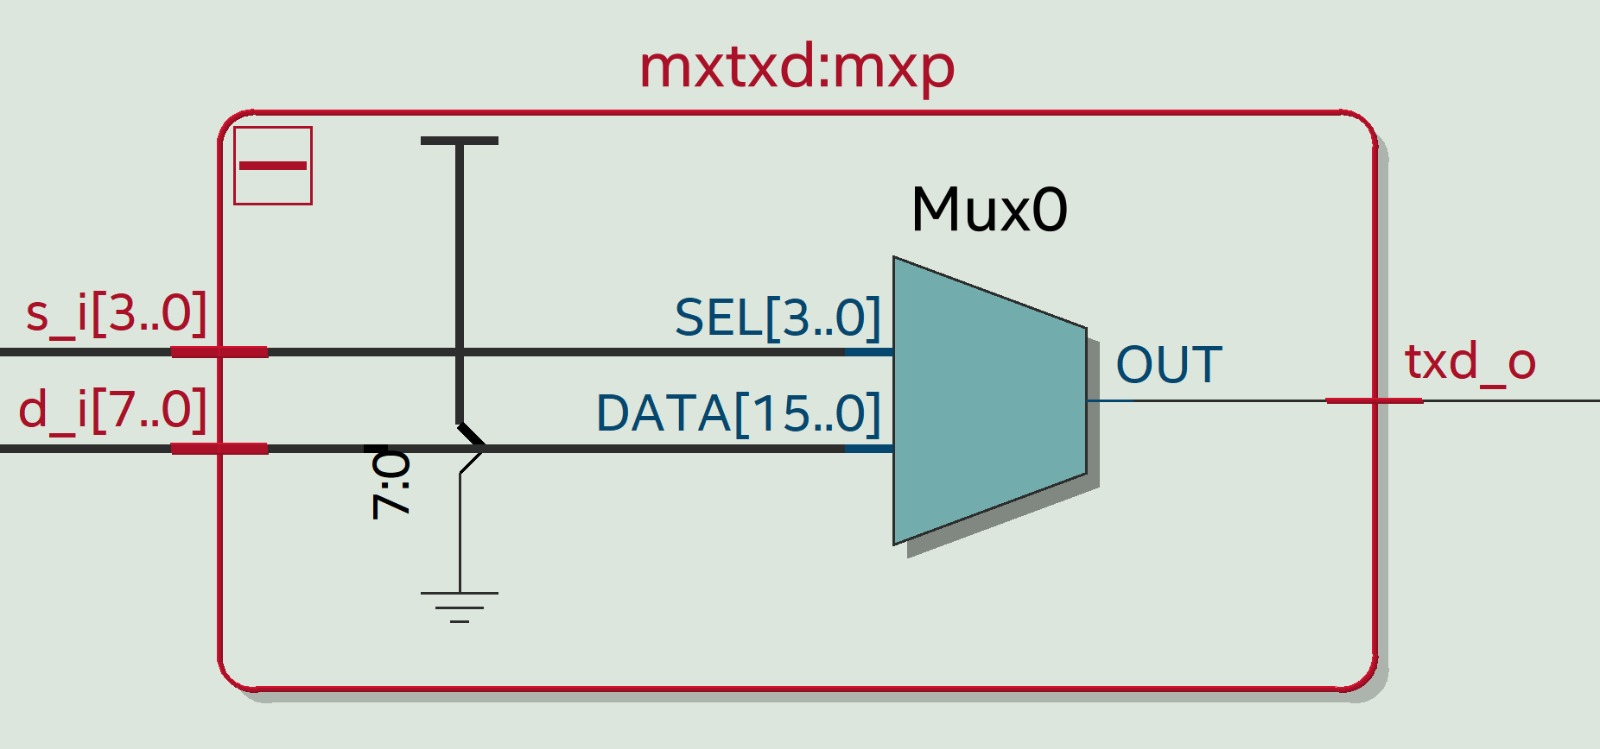
\includegraphics[scale=0.2]{../png/mxtxd_mxp.png}
	\newline
	fig:mxtxd\_mxp\\
\end{figure}
\begin{center}
	\begin{tabular}{ | p{2cm} | c | c | p{5cm} |}
		\hline
		\textbf{Pin} & \textbf{Direction} & \textbf{Width} & \textbf{Description} \\
		\hline
		s\_i & IN & X & Bit position \\
		\hline
		d\_i & IN & X & Bit vector \\
		\hline
		txd\_o & OUT & 1 & Txd, Serial Output \\
		\hline	
		
	\end{tabular}
\end{center} 
\subsection{Finite State Machine for Interface to S3}
\begin{figure}[h]
	\centering	
	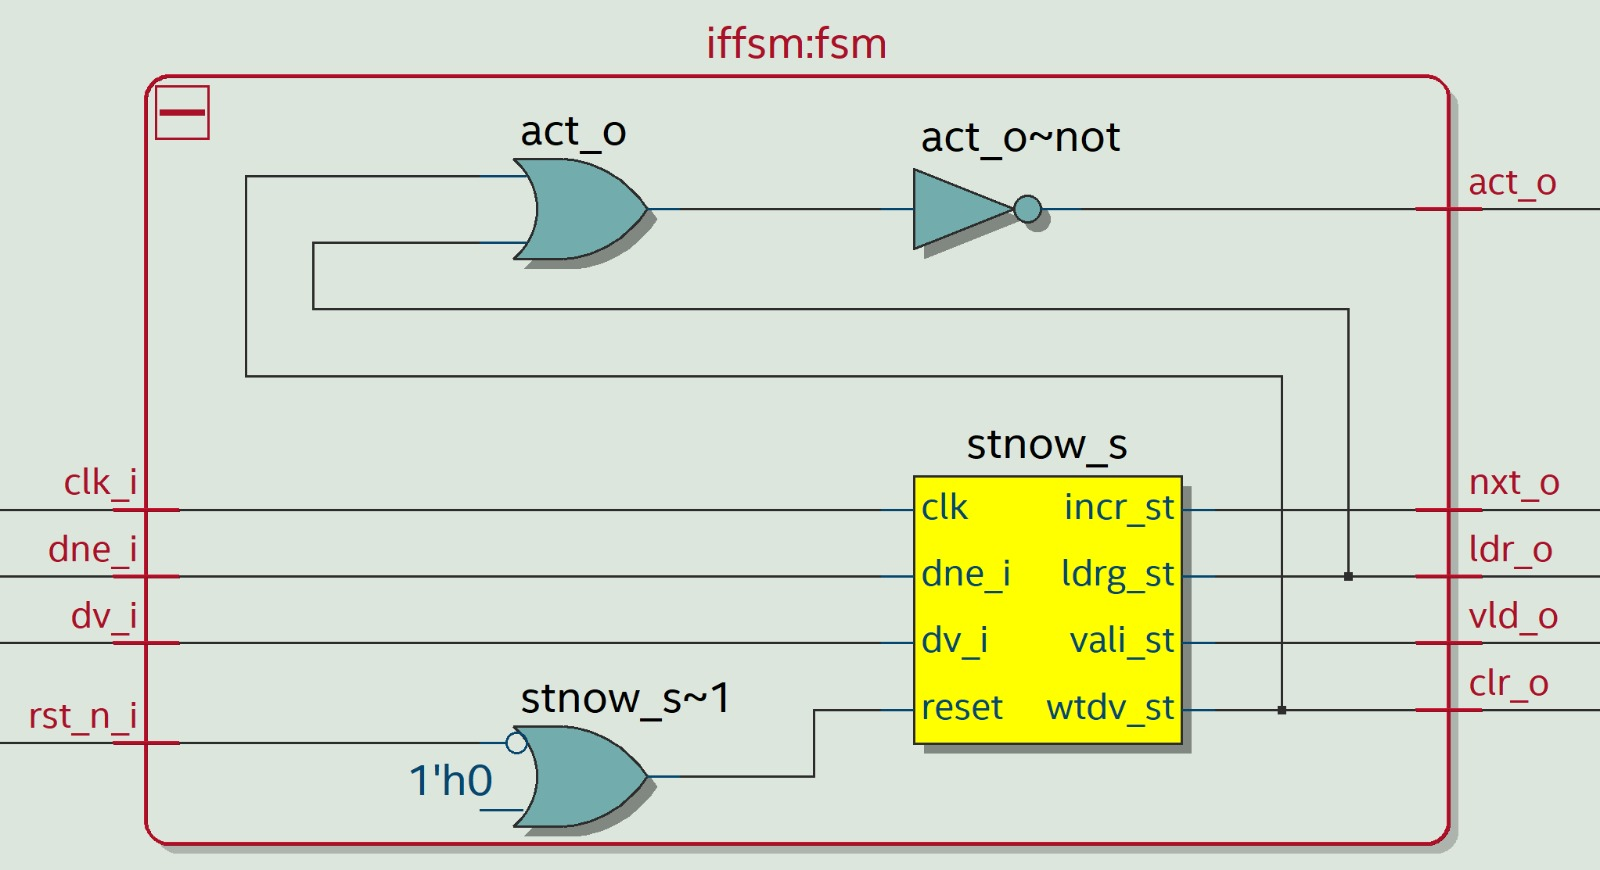
\includegraphics[scale=0.2]{../png/iffsm_fsm.png}
	\newline
	fig:iffsm\_fsm\\
\end{figure}
\begin{center}
	\begin{tabular}{ | p{2cm} | c | c | p{5cm} |}
		\hline
		\textbf{Pin} & \textbf{Direction} & \textbf{Width} & \textbf{Description} \\
		\hline
		rst\_n\_i & IN &  & Reset, active low \\
		\hline
		clk\_i & IN &  & Syscp, @ 12MHz \\
		\hline
		dv\_i & IN &  & Have new RTC or GPS-Data \\
		\hline
		dne\_i & IN &  & Last Bit transmitted \\
		\hline
		ldr\_o & OUT &  & Enable register load \\
		\hline
		act\_o & OUT &  & Transmission active \\
		\hline
		vld\_o & OUT &  & Data Bit valid \\
		\hline
		clr\_o & OUT &  & Clear Bit-Counters \\
		\hline
		nxt\_o & OUT &  & Next Bit, inc count \\
		\hline
		
	\end{tabular}
	\end{center}
\subsection{Multiplexer for Interface to S3}
\begin{figure}[h]
	\centering	
	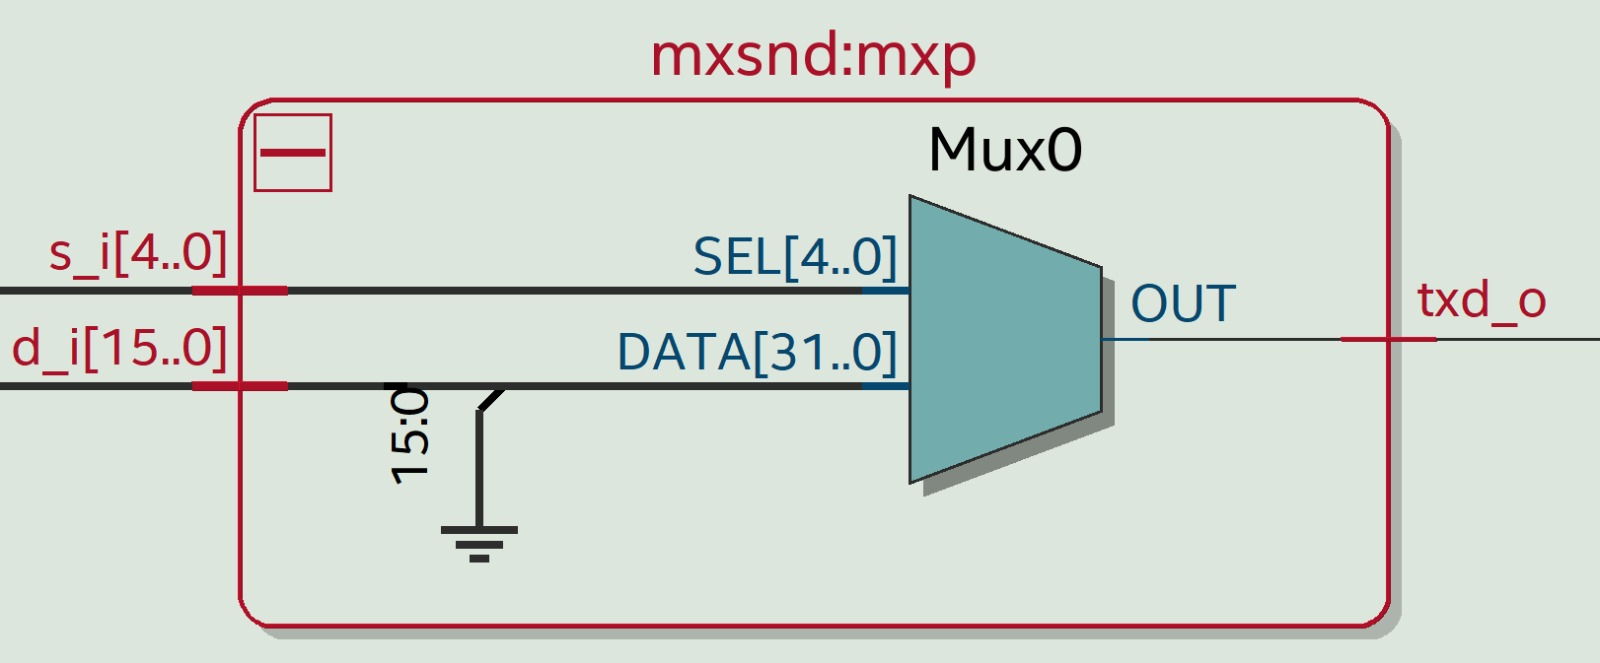
\includegraphics[scale=0.2]{../png/mxsnd_mxp.png}
	\newline
	fig:mxsnd\_mxp\\
\end{figure}
\begin{center}
	\begin{tabular}{ | p{2cm} | c | c | p{5cm} |}
		\hline
		\textbf{Pin} & \textbf{Direction} & \textbf{Width} & \textbf{Description} \\
		\hline
		s\_i & IN &  & Bit position \\
		\hline
		d\_i & IN &  &  Bit vector \\
		\hline	
		txd\_o & OUT &  & txd, Serial Output \\
		\hline
		
	\end{tabular}
\end{center}

\newpage

\section{State Diagrams}
The State Transition and the Output states of Uart,Control,Trigger and ifs\_3 are given below\\

\newpage

\subsection{Control Fsm}
\begin{figure}[h]
	\centering	
	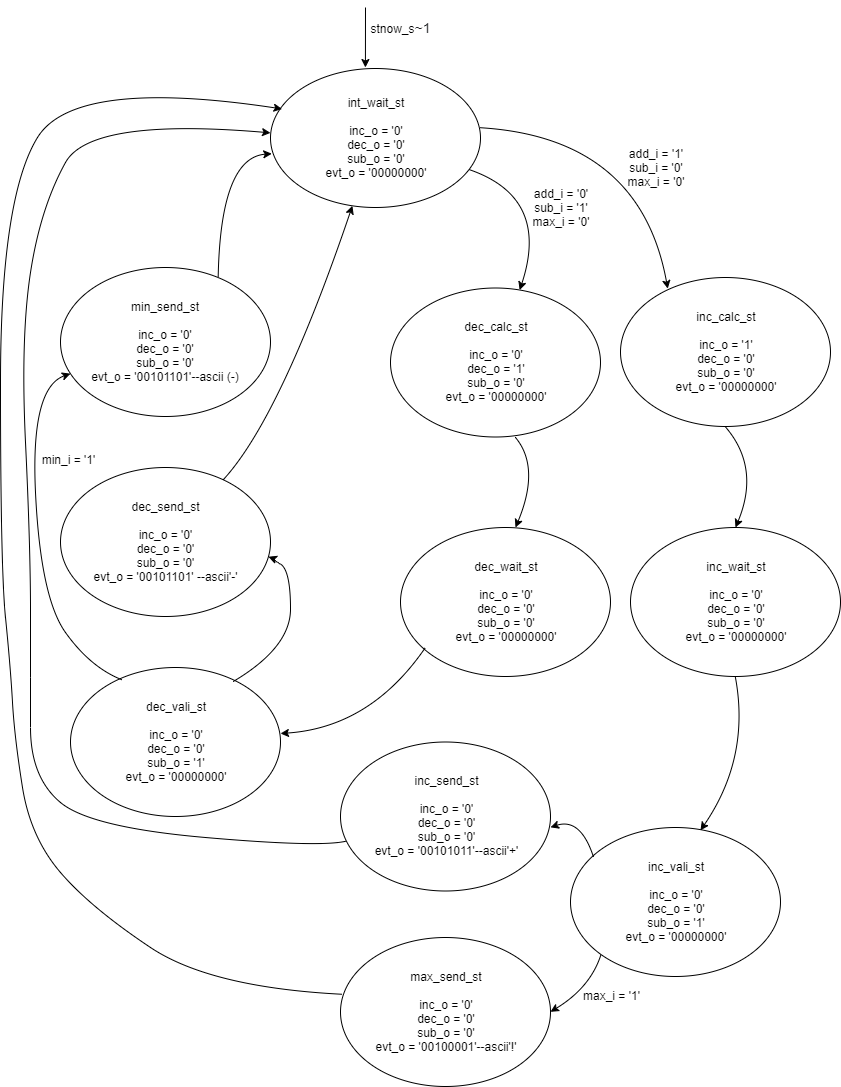
\includegraphics[scale=0.3]{../png/Control.png}
	\newline
	fig: Control FSM\\
\end{figure}
\begin{center}
 \begin{tabular}{| p{4cm} | p{7cm} |}
	 \hline
	 \textbf{State Name} & \textbf{Description} \\
	 \hline
	 ini\_wait\_st & wait until \\
	 \hline
	 inc\_clac\_st & send increase signal to headcounter \\
	 \hline
	 dec\_calc\_st & send decrease signal to headcounter \\
	 \hline
	 inc\_wait\_st & wait until headcount calculated \\
	 \hline
	 dec\_wait\_st & wait until headcount calculated \\
	 \hline
	 inc\_vali\_st & done calculating, check if max \\
	 \hline
	 dec\_vali\_st & done calculating, check if min \\
	 \hline
	 inc\_send\_st & start sending num and ascii \\
	 \hline
	 dec\_send\_st & start sending num and ascii \\
	 \hline
	 min\_send\_st & start sending num and ascii \\
	 \hline
	 max\_send\_st & start sending num and ascii \\
	 \hline
 \end{tabular}
\end{center}

\begin{center}
	\begin{tabular}{| p{2cm} | p{2cm} | p{11cm} |}
		\hline
		Source State& Destination State & Condition \\
		\hline
		ewt1\_st & ewt2\_st & (!s3\_i).(!s1\_i).(s2\_i) \\
		\hline
		ewt1\_st & ewt1\_st  & (!s3\_i).(!s1\_i).(!s3\_i)+(!s3\_i).(s1\_i)+(s3\_i) \\
		\hline
		ewt2\_st & ewt3\_st & (s3\_i).(!s1\_i).(!s2\_i)\\
		\hline
		ewt2\_st & ewt2\_st & (!s3\_i)+(s3\_i).(!s1\_i)+(s3\_i).(s1\_i)\\
		\hline
		ewt3\_st & init\_st & \\
		\hline
		init\_st & ewt1\_st & (!s3\_i).(s1\_i).(!s2\_i)\\
		\hline
		init\_st & lwt1\_st & (s3\_i).(!s1\_i).(!s2\_i)\\
		\hline
		init\_st & init\_st & (!s3\_i).(!s1\_i)+(!s3\_i).(s1\_i).(s2\_i)+(s3\_i).(!s3\_i).(s2\_i)+(s3\_i).(s1\_i)\\
		\hline	
		lwt1\_st & lwt2\_st & (!s3\_i).(!s1\_i).(!s2\_i)\\
		\hline	
		lwt1\_st & lwt1\_st & (!s3\_i).(!s1\_i).(!s2\_i)+ (!s3\_i).(s1\_i)+(s3\_i)\\
		\hline
		lwt2\_st & lwt3\_st & (!S3\_i).(s1\_i).(!s2\_i) \\
		\hline
		lwt2\_st & lwt2\_st & (!s3\_i).(!s1\_i)+(!s3\_i)(s1\_i).(s2\_i)+(s3\_i) \\
		\hline
		lwt3\_st & init\_st  & \\
		\hline	
	\end{tabular}
\end{center}

\newpage

\subsection{Trigger Fsm}
\begin{figure}[h]
	\centering	
	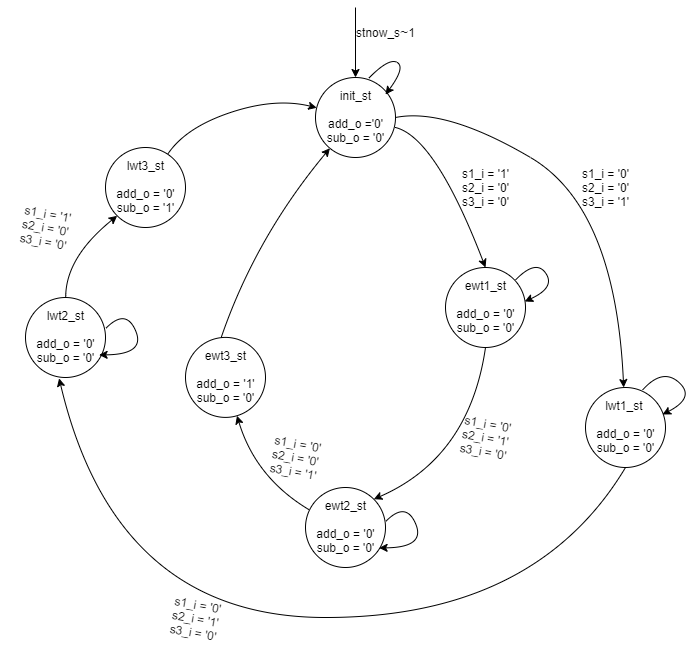
\includegraphics[scale=0.4]{../png/Trigger.png}
	\newline
	fig: Trigger FSM\\
\end{figure}
\begin{center}
 \begin{tabular}{| p{4cm} | p{7cm} |}
	 \hline
	 \textbf{State Name} & \textbf{Description} \\
	 \hline
	 init\_st & wait for either sensor 1 or sensor 2 triggered \\
	 \hline
	 ewt1\_st & someone entering, sensor 1 triggered wait for sensor 2 \\
	 \hline
	 lwt1\_st & someone leaving, sensor 3 triggered wait for sensor 2 \\
	 \hline
	 ewt2\_st & someone entering, sensor 2 triggered wait for sensor 3 \\
	 \hline
	 lwt2\_st & someone leaving, sensor 2 triggered wait for sensor 1 \\
	 \hline
	 ewt3\_st & someone entering, sensor 3 triggered -> back to init \\
	 \hline
	 lwt3\_st & someone leaving, sensor 1 triggered -> back to init \\
	 \hline
 \end{tabular}
\end{center}
\begin{center}
	\begin{tabular}{| p{2cm} | p{2cm} | p{11cm} |}
		\hline
		Source State& Destination State & Condition \\
		\hline	
		
			
	\end{tabular}	
\end{center}

\newpage

\subsection{Uart Fsm}
\begin{figure}[h]
	\centering	
	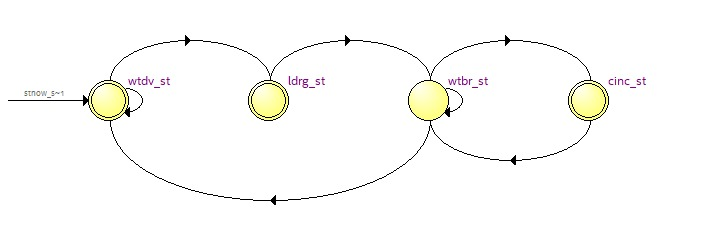
\includegraphics[scale=0.5]{../png/Uart.png}
	\newline
	fig: Uart FSM\\
\end{figure}
\begin{center}
 \begin{tabular}{| p{4cm} | p{7cm} |}
	 \hline
	 \textbf{State Name} & \textbf{Description} \\
	 \hline
	 wtdv\_st & wait until data valid \\
	 \hline
	 ldrg\_st & load data in register \\
	 \hline
	 wtbr\_st & wait till baud rate is 1 or goto wtdv when done transmitting \\
	 \hline
	 cinc\_st & get next bit (increment counter) \\
	 \hline
 \end{tabular}
\end{center}
\begin{center}
	\begin{tabular}{| p{2cm} | p{2cm} | p{11cm} |}
		\hline
		Source State& Destination State & Condition \\
		\hline	
		
		
	\end{tabular}	
\end{center}

\newpage

\subsection{ifs\_3 Fsm}
\begin{figure}[h]
	\centering	
	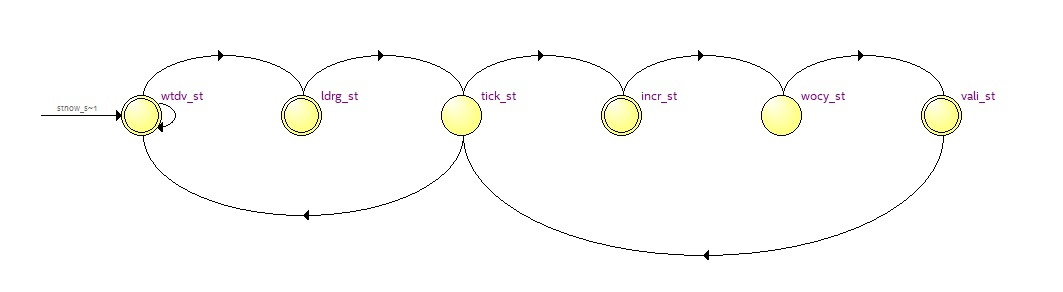
\includegraphics[scale=0.4]{../png/ifs_3.png}
	\newline
	fig: ifs\_3 FSM\\
\end{figure}
\begin{center}
 \begin{tabular}{| p{4cm} | p{7cm} |}
	 \hline
	 \textbf{State Name} & \textbf{Description} \\
	 \hline
	 wtdv\_st & wait until data valid \\
	 \hline
	 ldrg\_st & load data in register \\
	 \hline
	 tick\_st & check if done, else go on \\
	 \hline
	 incr\_st & get next bit (increment counter) \\
	 \hline
	 wocy\_st & wait one clock cycle \\
	 \hline
	 vali\_st & send validation bit \\
	 \hline
 \end{tabular}
\end{center}
\begin{center}
	\begin{tabular}{| p{2cm} | p{2cm} | p{11cm} |}
		\hline
		Source State& Destination State & Condition \\
		\hline	
		
		
	\end{tabular}	
\end{center}

\newpage

\chapter{PC Program}

\begin{center}
	\begin{tabular}{|l|c|c|r|}
		\hline
		\textbf{Event} & \textbf{Beep One} & \textbf{Beep Two} & \textbf{Description} \\
		\hline
		Enter & LOW & HIGH & Someone entered the room \\
		\hline
		Leave & HIGH & LOW & Someone left the room \\
		\hline
		Stop & MEDIUM & MEDIUM & The room is full \\
		\hline
	\end{tabular}
\end{center}

\end{document}
